\chapter{Results}
\label{chapter:results}
In this chapter we will implement all the models described before: constant volatility, Dupire's local volatility, Heston's stochastic volatility and both static and dynamic SABR models.

With the exception of Dupire's local volatility, will perform the calibration described in section \ref{section:Model Calibration} for all models: we will minimize the cost function in eq. \eqref{cost} with the weight function shown in eq. \eqref{weight}. The model values for the implied volatilities, $\sigma_{imp,\mathrm{mdl}}$, will be obtained through the closed form solutions for each of the models. We will apply the CMA-ES optimization algorithm to find the optimal solution.

To validate the models' closed-form solutions, after finding the optimal parameters we will input them into a Monte Carlo pricer (adapted to each model), and calculate the simulated option price with each model's calibrated parameters. This price will then be converted into an implied volatility (using eq.\eqref{impvolform}) in order for the simulation to be comparable to the data and the closed form solutions. To better grasp the behavior of the simulations we will repeat them a large number of times, $N_{\mathrm{reps}}$, averaging the results to produce a function - henceforth named \emph{simulated function} -  and extracting from them the 90\% confidence intervals of the simulations - these confidence intervals are obtained by sorting the simulated implied volatilities for each strike and extracting both the 90\% highest and the 10\% lowest.


We will fit all our functions to a dataset of implied volatilities for European options with different maturities and strike prices. This data was kindly provided by \emph{BNP Paribas} and is shown in Appendix \ref{chapter:mktdata}.


For the case of Dupire's local volatility, because it is nonparametric, no calibration is required. Instead we must perform an interpolation in order to find the implied volatility surface from the data mentioned before and, with it, find the local volatility function. From this, we can easily obtain the prices of European options from the Monte Carlo pricer described in subsections \ref{subsection:Simulating stock prices} and \ref{subsection:Pricing options from simulations}. These prices (and their implied volatilities) can then be compared to their true market values. As for the stochastic volatility models above, we will also run the Monte Carlo pricer a large number of times, $N_{\mathrm{reps}}$, to produce the simulated function and its 90\% confidence intervals.


In order for the models to be comparable, we need to make sure that the same global parameters are used in all the adjustments and simulations, namely the initial stock price, $S_0$, the risk-free interest rate, $r$, the time step size (used in the Monte Carlo simulations), $\Delta t$, the number of pricer repetitions (to be averaged, producing the expected simulated function and the confidence intervals), $N_{\mathrm{reps}}$, and the number of paths simulated, $N_{\mathrm{paths}}$. Their values are shown in \autoref{tab:defaultparam}.
\begin{table}[H]
    \centering
        \renewcommand{\arraystretch}{0.8}
\begin{tabular}{@{}lcccr@{}}
\toprule
$S_0$($\EUR$) & $r$($\SI{}{\per\year}$) & $\Delta t$(days) & $N_{\mathrm{paths}}$ & $N_{\mathrm{reps}}$ \\ \midrule
1 & 0 & 0.5 & 100 000 & 100\\
\bottomrule
\end{tabular}
  \caption[Parameters used throughout all simulations.]{Parameters used throughout all simulations.}
  \label{tab:defaultparam}
\end{table}

The Monte Carlo pricers of each model will then be modified to price Barrier options instead of the European options used in the calibration. These results will be compared with one another, though no validation is possible due to a lack of data.



\section{Constant Volatility Model}
To find how well our models perform, we need some reference against which to compare them. One clear possibility is to assume a constant volatility throughout the options' duration, since this is the simplest possible case.

The equation that generates each stock price path is therefore given by
\begin{equation}
dS(t)=rS(t)dt+\sigma S(t)dW(t).
\end{equation}

Because we are fitting the volatility function - which, in this case, is a constant value - to a set of volatility data - which is not constant - these adjustments are expected to badly represent the data. Any other minimally decent model is expected to outperform this constant volatility benchmark.

With this constant volatility model, we can choose to fit the datasets with different maturities independently of one another or together in a single coupled dataset. In other words, we can do several fits, one for each maturity, or a single one, for all maturities together. The former will be useful when benchmarking the Static SABR model, since for that model the adjustments will also be performed independently (Static SABR performs badly for multiple maturities). The latter will be more appropriate when studying the remaining models - Dupire, Heston and Dynamic SABR - since these fit the whole implied volatility surface (i.e. multiple maturities together). Thus, both versions will be implemented and briefly studied.


\newpage
\subsection{Independent Fits}
We begin by presenting the results of fitting a constant volatility function to the sets of data with different maturities \emph{independently}.


In \autoref{fig:ConstVol} we show the plots of each fit along with the provided market data. We also present the simulated functions and the simulations' confidence intervals.
\begin{figure}[H]
  \begin{subfigmatrix}{2}
    \subfigure[$T=21$ days]{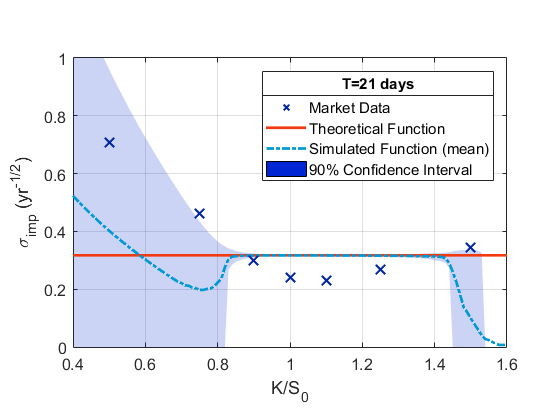
\includegraphics[width=0.49\linewidth,trim={0.25cm 0.45cm 1.1cm 1.4cm},clip]{ConstVol1.png}}
    \subfigure[$T=42$ days]{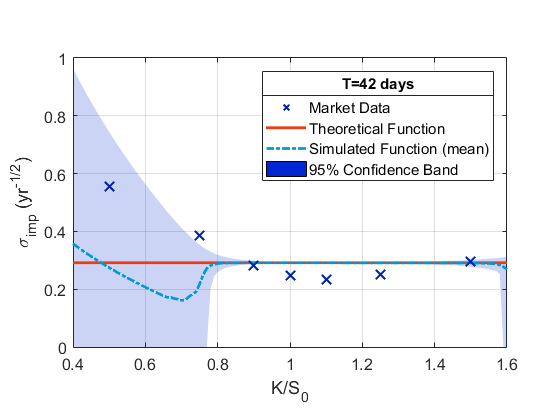
\includegraphics[width=0.49\linewidth,trim={0.25cm 0.45cm 1.1cm 1.4cm},clip]{ConstVol2.png}}
    \subfigure[$T=63$ days]{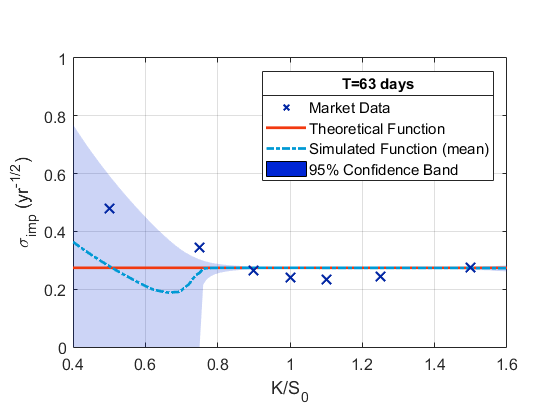
\includegraphics[width=0.49\linewidth,trim={0.25cm 0.45cm 1.1cm 1.4cm},clip]{ConstVol3.png}}
    \subfigure[$T=126$ days]{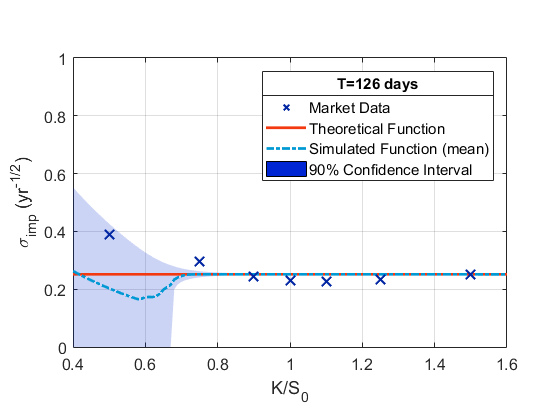
\includegraphics[width=0.49\linewidth,trim={0.25cm 0.45cm 1.1cm 1.4cm},clip]{ConstVol4.png}}
  \end{subfigmatrix}
  \caption[Implied volatility functions fitted independently to the implied volatility data for different maturities under constant volatility model, plotted with their respective Monte Carlo simulated functions along with their confidence intervals.]{Implied volatility functions (red lines) fitted \emph{independently} to the implied volatility data (crosses) for different maturities under constant volatility model, plotted with their respective Monte Carlo simulated functions (light-blue dot-dashed lines) along with their 90\% confidence intervals (blue region).}
  \label{fig:ConstVol}
\end{figure}

The fitted parameter, which, in this case, is only the constant implied volatility, is presented in \autoref{tab:ConstVolPar} for each of the maturities, along with the cost function's value (eq.\eqref{cost}) under this (fitted) model.

\begin{table}[H]
    \centering
        \renewcommand{\arraystretch}{0.8}
\begin{tabular}{@{}lcr@{}}
\toprule
$T$ (days) & $\sigma_{imp,\mathrm{mdl}}$ ($\SI{}{\year\tothe{-1/2}}$) & Cost \\ \midrule
21 & 0.3174 & 0.0635 \\
42 & 0.2918 & 0.0282 \\
63 & 0.2742 & 0.0164 \\
126& 0.2518 & 0.0069 \\
\bottomrule
\end{tabular}
  \caption[Fitted parameters for each maturity (fitted independently) under constant volatility model.]{Fitted parameters for each maturity (fitted independently) under constant volatility model.}
  \label{tab:ConstVolPar}
\end{table}


\begin{table}[H]
\centering
\renewcommand{\arraystretch}{0.8}
\begin{tabular}{@{}ccccSccS@{}}
\toprule
$T$(days) & $K$($\EUR$) & $\sigma_{i,\mathrm{mkt}}$($\SI{}{\year\tothe{-0.5}}$) &  $\sigma_{i,\mathrm{mdl}}$($\SI{}{\year\tothe{-0.5}}$) & \multicolumn{1}{c}{$\mathrm{Error}_{\sigma}(\%)$} & $C_{\mathrm{mkt}}$($\EUR$)&$C_{\mathrm{mdl}}$($\EUR$)& \multicolumn{1}{c}{$\mathrm{Error}_{C}(\%)$}\\ \midrule
\multirow{7}{*}{21} & 0.50 & 0.7082 & \multirow{7}{*}{0.3174} & 55.2 & 0.50001 & 0.50000 & 0.003 \\
&0.75 & 0.4632 &  & 31.5 & 0.25065 & 0.25002 & 0.3 \\
&0.90 & 0.2989 &  & 6.2 & 0.10439 & 0.10540 & 1.0 \\
&1.00 & 0.2425 &  & 30.9 & 0.02792 & 0.03654 & 30.9 \\
&1.10 & 0.2314 &  & 37.1 & 2.42$\times10^{-3}$ & 7.41$\times10^{-3}$ & 205.9 \\
&1.25 & 0.2699 &  & 17.6 & 5.34$\times10^{-5}$ & 25.01$\times10^{-5}$ & 367.9 \\
&1.50 & 0.3433 &  & 7.5 & 5.75$\times10^{-7}$ & 1.12$\times10^{-7}$ & 80.5 \\\midrule
\multirow{7}{*}{42}&0.50 & 0.5556 & \multirow{7}{*}{0.2918} & 47.5 & 0.50005 & 0.50000 & 0.01 \\
&0.75 & 0.3876 &  & 24.7 & 0.25186 & 0.25027 & 0.6 \\
&0.90 & 0.2824 &  & 3.3 & 0.11069 & 0.11166 & 0.9 \\
&1.00 & 0.2461 &  & 18.6 & 0.04006 & 0.04749 & 18.5 \\
&1.10 & 0.2354 &  & 23.9 & 8.52$\times10^{-3}$ & 15.00$\times10^{-3}$ & 75.9 \\
&1.25 & 0.2525 &  & 15.6 & 6.21$\times10^{-4}$ & 15.75$\times10^{-4}$ & 153.8 \\
&1.50 & 0.2968 &  & 1.7 & 1.58$\times10^{-5}$ & 1.24$\times10^{-5}$ & 21.4 \\\midrule
\multirow{7}{*}{63}&0.50 & 0.4789 &\multirow{7}{*}{0.2742}  & 42.7 & 0.50009 & 0.50000 & 0.02 \\
&0.75 & 0.3452 &  & 20.6 & 0.25296 & 0.25077 & 0.9 \\
&0.90 & 0.2658 &  & 3.2 & 0.11533 & 0.11650 & 1.0 \\
&1.00 & 0.2401 &  & 14.2 & 0.04787 & 0.05465 & 14.2 \\
&1.10 & 0.2330 &  & 17.7 & 0.01421 & 0.02069 & 45.5 \\
&1.25 & 0.2438 &  & 12.5 & 1.80$\times10^{-3}$ & 3.33$\times10^{-3}$ & 85.1 \\
&1.50 & 0.2749 &  & 0.3 & 7.66$\times10^{-5}$ & 7.44$\times10^{-5}$ & 2.9 \\\midrule
\multirow{7}{*}{126}&0.50 & 0.3878 &  \multirow{7}{*}{0.2518}& 35.1 & 0.50035 & 0.50000 & 0.07 \\
&0.75 & 0.2954 &  & 14.7 & 0.25694 & 0.25344 & 1.4 \\
&0.90 & 0.2444 &  & 3.1 & 0.12716 & 0.12882 & 1.3 \\
&1.00 & 0.2295 &  & 9.7 & 0.06467 & 0.07094 & 9.7 \\
&1.10 & 0.2269 &  & 11.0 & 0.02862 & 0.03488 & 21.9 \\
&1.25 & 0.2340 &  & 7.6 & 7.57$\times10^{-3}$ & 9.98$\times10^{-3}$ & 31.8 \\
&1.50 & 0.2521 &  & 0.1 & 8.58$\times10^{-4}$ & 8.51$\times10^{-4}$ & 0.8 \\
\bottomrule
\end{tabular}
  \caption[Comparison between fitted results (fitted independently) and original data under constant volatility model.]{Comparison between fitted functions (fitted independently) and original data under constant volatility model.}
  \label{tab:CV}
\end{table}

By observing the fit results in \autoref{tab:ConstVolPar} we see that the cost function decreases with the maturity. This is indeed what is expected, since the implied volatility surface becomes flatter as maturity increases, as can be seen from the market data (and also as we can see in \autoref{fig:DupImpV}), making the constant volatility function a better approximation in such cases, and decreasing the cost function's value.


One other property that we can observe is that the constant implied volatility also decreases with maturity. The reason behind this is the simple fact that earlier maturities contain higher implied volatilities, which pull the constant volatility function upwards.


We now focus on the simulated results in \autoref{fig:ConstVol}.

First, we can see that the theoretical functions (full red lines) clearly don't represent the market data. This is indeed what is expected. After all, if a constant volatility model was enough to price options, the more complex models would not be needed.

Secondly, by comparing the theoretical and simulated functions, we must note that the simulation performs extremely well for strikes near $S_0$. Notice that the simulated function (dot-dashed blue line) perfectly follows the constant volatility theoretical result (full red line) in this region, with the confidence intervals collapsed into the simulated function indicating that all simulations produced the same result. This suggests that the simulation is working as expected.

Thirdly, we notice that on the earliest maturity (i.e. 21 days), for strikes much larger than $S_0$ (e.g. $K=1.5S_0$), the simulated implied volatilities go to zero, even though they should remain constant. The reason behind this has already been discussed in subsection \ref{subsection:Pricing options from simulations} and relates to the very, very small number of paths that reach such high strikes and end up contributing to the option price (which is then converted to an implied volatility). For the case of strike $K=1.5S_0$, and maturity $T=21$ days, the number of paths that reach the strike is indeed approximately 0.25 - sometimes a single path is able to breach this strike, but usually none do. This problem is not observed for the remaining maturities for the simple reason that, because they are given more time to evolve, more paths are able to reach these high strikes.

Finally we must discuss the large confidence intervals for strikes lower than $S_0$, occurring over all maturities. To explain this we require the information presented in \autoref{fig:ImpVolPrice}, relating the implied volatility with the option's market price. We saw that the implied volatility was extremely sensitive to option prices very close to their lower bounds, $S_0-Ke^{-rT}$. If we now look, for example, at the market price of the option with strike $K=\SI{0.5}{\EUR}$ and maturity $T=21$ days, which is $C=\SI{0.500013}{\EUR}$, and we compare it with its lower bound, $S_0-Ke^{-rT}=\SI{0.5}{\EUR}$, we can clearly see that they are extremely close, with a difference of only $0.0026\%$. We can then conclude that, in this case, we are in the extremely high sensitivity region of the implied volatility functions shown in \autoref{fig:ImpVolPrice}.
The Monte Carlo pricer behaves very well for the lower strikes since a very large number of paths contribute to the option price (the opposite of what we described before for high strikes). Despite this, because there will always be some noise associated with the simulations, the generated price is sure to present some very slight variation when executed multiple times, which is enough to cause some of the simulated implied volatilities to go to approximately zero (or to increase), which explains the large confidence intervals. For options with strikes near $S_0$ and above the market option price is much farther from its lower bound, so that we are above the high sensitivity region. Indeed, the lower bound of options with strikes equal to or above $S_0$ is 0 (assuming interest rate $r=0$).

These two last problems are not inherent to the constant volatility model. Indeed they will be observed, to some extent, in all the models we will study next.




\newpage

\subsection{Dependent Fits}
We now present the results obtained from the adjustment of a constant volatility function to all the implied volatility data, regardless of maturity.

In \autoref{fig:ConstVol2} are shown the theoretical and simulated functions as well as the provided market data.
\begin{figure}[H]
  \begin{subfigmatrix}{2}
    \subfigure[$T=21$ days]{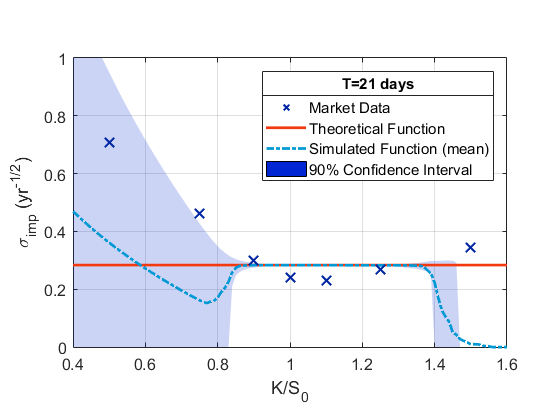
\includegraphics[width=0.49\linewidth,trim={0.25cm 0.45cm 1.1cm 1.4cm},clip]{ConstVol12.png}}
    \subfigure[$T=42$ days]{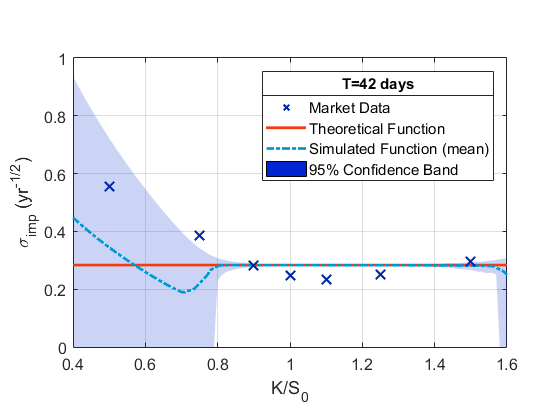
\includegraphics[width=0.49\linewidth,trim={0.25cm 0.45cm 1.1cm 1.4cm},clip]{ConstVol22.png}}
    \subfigure[$T=63$ days]{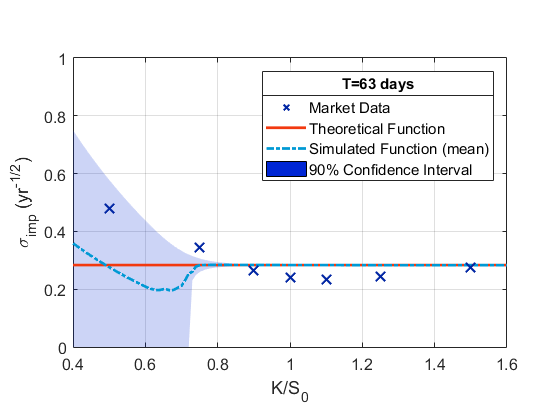
\includegraphics[width=0.49\linewidth,trim={0.25cm 0.45cm 1.1cm 1.4cm},clip]{ConstVol32.png}}
    \subfigure[$T=126$ days]{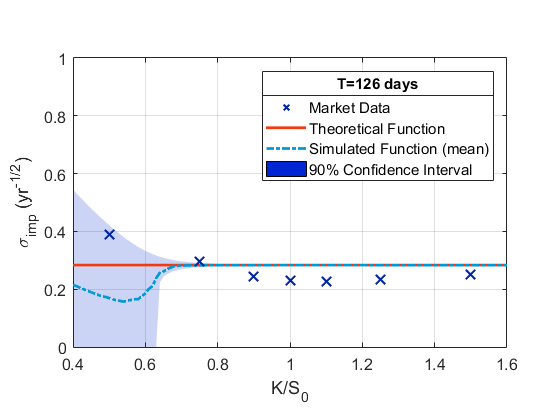
\includegraphics[width=0.49\linewidth,trim={0.25cm 0.45cm 1.1cm 1.4cm},clip]{ConstVol42.png}}
  \end{subfigmatrix}
  \caption[Implied volatility functions fitted simultaneously to the implied volatility data for different maturities under constant volatility model, plotted with their respective Monte Carlo simulated functions along with their confidence intervals.]{Implied volatility functions (red lines) fitted \emph{simultaneously} to the implied volatility data (crosses) for different maturities under constant volatility model, plotted with their respective Monte Carlo simulated functions (light-blue dot-dashed lines) along with their 90\% confidence intervals (blue region).}
  \label{fig:ConstVol2}
\end{figure}

The fitted implied volatility is represented in \autoref{tab:ConstVolPar2} as well as the cost function's value.
\begin{table}[H]
    \centering
        \renewcommand{\arraystretch}{0.8}
\begin{tabular}{@{}lr@{}}
\toprule
 $\sigma_{imp,\mathrm{mdl}}$ ($\SI{}{\year\tothe{-1/2}}$) & Cost \\ \midrule
0.2838 & 0.1248 \\
\bottomrule
\end{tabular}
  \caption[Fitted parameters for all maturities (fitted simultaneously) under constant volatility model.]{Fitted parameters for all maturities (fitted simultaneously) under constant volatility model.}
  \label{tab:ConstVolPar2}
\end{table}


\begin{table}[H]
\centering
\renewcommand{\arraystretch}{0.8}
\begin{tabular}{@{}ccccSccS@{}}
\toprule
$T$(days) & $K$($\EUR$) & $\sigma_{i,\mathrm{mkt}}$($\SI{}{\year\tothe{-0.5}}$) &  $\sigma_{i,\mathrm{mdl}}$($\SI{}{\year\tothe{-0.5}}$) & \multicolumn{1}{c}{$\mathrm{Error}_{\sigma}(\%)$} & $C_{\mathrm{mkt}}$($\EUR$)&$C_{\mathrm{mdl}}$($\EUR$)& \multicolumn{1}{c}{$\mathrm{Error}_{C}(\%)$}\\ \midrule
\multirow{7}{*}{21} & 0.50 & 0.7082 & \multirow{7}{*}{0.2838} & 59.9 & 0.50001 & 0.50000 & 0.003 \\
 & 0.75 & 0.4632 &  & 38.7 & 0.25065 & 0.25000 & 0.3 \\
 & 0.90 & 0.2989 &  & 5.0 & 0.10439 & 0.10364 & 0.7 \\
 & 1.00 & 0.2425 &  & 17.0 & 0.02792 & 0.03267 & 17.0 \\
 & 1.10 & 0.2314 &  & 22.6 & 2.42$\times10^{-3}$ & 5.19$\times10^{-3}$ & 114.4 \\
 & 1.25 & 0.2699 &  & 5.1 & 5.34$\times10^{-5}$ & 8.98$\times10^{-5}$ & 67.9 \\
 & 1.50 & 0.3433 &  & 17.3 & 5.75$\times10^{-7}$ & 0.07$\times10^{-7}$ & 98.8 \\\midrule
\multirow{7}{*}{42} & 0.50 & 0.5556 & \multirow{7}{*}{0.2838} & 48.9 & 0.50005 & 0.50000 & 0.01 \\
 & 0.75 & 0.3876 &  & 26.8 & 0.25186 & 0.25021 & 0.7 \\
 & 0.90 & 0.2824 &  & 0.5 & 0.11069 & 0.11084 & 0.1 \\
 & 1.00 & 0.2461 &  & 15.3 & 0.04006 & 0.04620 & 15.3 \\
 & 1.10 & 0.2354 &  & 20.6 & 8.52$\times10^{-3}$ & 14.02$\times10^{-3}$ & 64.5 \\
 & 1.25 & 0.2525 &  & 12.4 & 6.21$\times10^{-4}$ & 13.36$\times10^{-4}$ & 115.3 \\
 & 1.50 & 0.2968 &  & 4.4 & 1.58$\times10^{-5}$ & 0.83$\times10^{-5}$ & 47.6 \\\midrule
\multirow{7}{*}{63} & 0.50 & 0.4789 & \multirow{7}{*}{0.2838} & 40.7 & 0.50009 & 0.50000 & 0.02 \\
 & 0.75 & 0.3452 && 17.8 & 0.25296 & 0.25097 & 0.8 \\
 & 0.90 & 0.2658 && 6.8 & 0.11533 & 0.11786 & 2.2 \\
 & 1.00 & 0.2401 && 18.2 & 0.04787 & 0.05656 & 18.2 \\
 & 1.10 & 0.2330 && 21.8 & 0.01421 & 0.02227 & 56.7 \\
 & 1.25 & 0.2438 && 16.4 & 1.80$\times10^{-3}$ & 3.93$\times10^{-3}$ & 118.2 \\
 & 1.50 & 0.2749 && 3.2 & 7.66$\times10^{-5}$ & 10.87$\times10^{-5}$ & 42.0 \\\midrule
\multirow{7}{*}{126} & 0.50 & 0.3878 & \multirow{7}{*}{0.2838} & 26.8 & 0.50035 & 0.50001 & 0.1 \\
 & 0.75 & 0.2954 && 3.9 & 0.25694 & 0.25589 & 0.4 \\
 & 0.90 & 0.2444 && 16.1 & 0.12716 & 0.13611 & 7.0 \\
 & 1.00 & 0.2295 && 23.7 & 0.06467 & 0.07992 & 23.6 \\
 & 1.10 & 0.2269 && 25.1 & 0.02862 & 0.04317 & 50.8 \\
 & 1.25 & 0.2340 && 21.3 & 7.57$\times10^{-3}$ & 14.99$\times10^{-3}$ & 98.0 \\
 & 1.50 & 0.2521 && 12.6 & 8.58$\times10^{-4}$ & 19.67$\times10^{-4}$ & 129.3 \\
\bottomrule
\end{tabular}
  \caption[Comparison between fitted results (fitted simultaneously) and original data under constant volatility model.]{Comparison between fitted functions (fitted simultaneously) and original data under constant volatility model.}
  \label{tab:CV2}
\end{table}


First, when we compare the implied volatility fitted to all the maturities with the results of the independent fits (in \autoref{tab:ConstVolPar}) we see that the former is actually the average of the latter. \hl{why?}

If we now compare the cost function values, we see that the cost of the dependent fit ($0.1248$), is actually larger than the sum of cost of the independent fits ($0.0635+0.0282+0.0164+0.0069=0.1150$). This is indeed expected: when fitting all maturities at once, the optimizer will find the implied volatility that minimizes the cost for all maturities, which will not be the one that minimizes the cost of each single maturity, so that the sum of the errors is higher.

As for the plots in \autoref{fig:ConstVol2} they look very similar to those in \autoref{fig:ConstVol}, so not much more can be added regarding their analysis.





\newpage
\section{Dupire Model}
The stochastic differential equation for the stock price paths under the local volatility model was hypothesized to be given by
\begin{equation}\label{dupmodds}
dS(t)=rS(t)dt+\sigma(S,t)S(t)dW(t),
\end{equation}
\noindent where $\sigma(S,t)$ can be obtained through Dupire's model, defined in subsection \ref{subsection:Dupire}, which is given by
\begin{equation}
\sigma(S,t)=\sqrt{\frac{\displaystyle\sigma_{imp}^2+2t\sigma_{imp}\pdv{\sigma_{imp}}{T}+2rSt\sigma_{imp}\pdv{\sigma_{imp}}{K}}{\displaystyle\left(1+Sd_1\sqrt{t}\pdv{\sigma_{imp}}{K}\right)^2+S^2t\sigma_{imp}\left(\pdv{^2\sigma_{imp}}{K^2}-d_1\left(\pdv{\sigma_{imp}}{K}\right)^2\sqrt{t}\right)}},
\end{equation}
\noindent where $d_1$ is defined as
\begin{equation}
d_1=\frac{\log(S_0/S)+\left(r+\frac{1}{2}\sigma_{imp}^2\right)t}{\sigma_{imp}\sqrt{t}}.
\end{equation}

As we mentioned in Section \ref{section:Surface Interpolation (Dupire)}, we must produce the implied volatility surface from the market data using an interpolation algorithm. Applying the Delaunay triangulation defined earlier, we obtain the implied volatility surface shown in \autoref{fig:DupImpV}, along with its contour plot.
From this surface we can easily extract (numerically) the gradients required for the local volatility formula.



\begin{figure}[H]
  \begin{subfigmatrix}{2}
    \subfigure[$\sigma_{imp}$ surface]{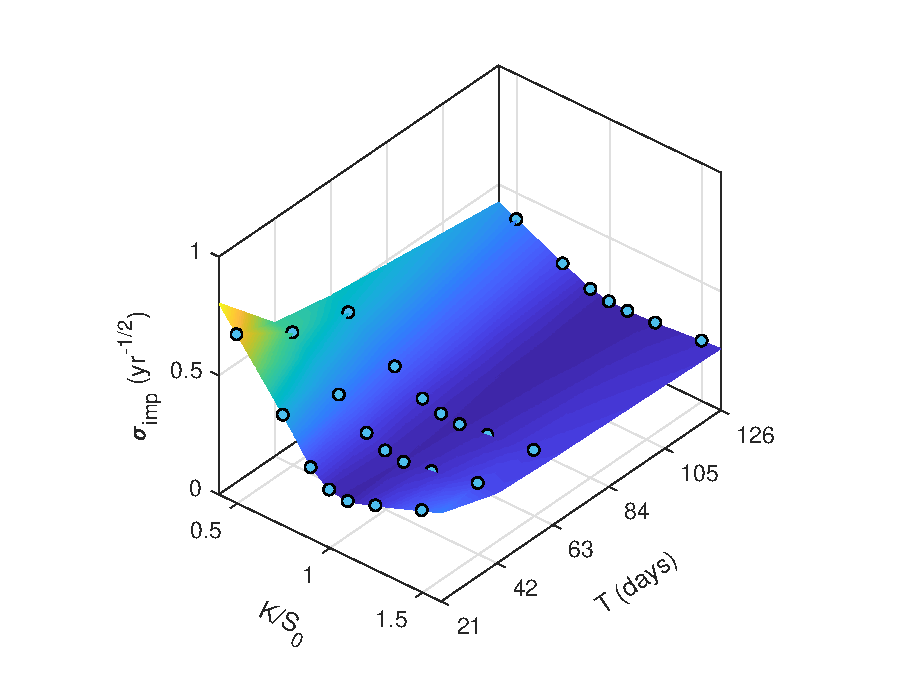
\includegraphics[width=0.49\linewidth,trim={1.7cm 0.45cm 2.cm 0.85cm},clip]{ImpliedV.eps}}
    \subfigure[$\sigma_{imp}$ contour plot]{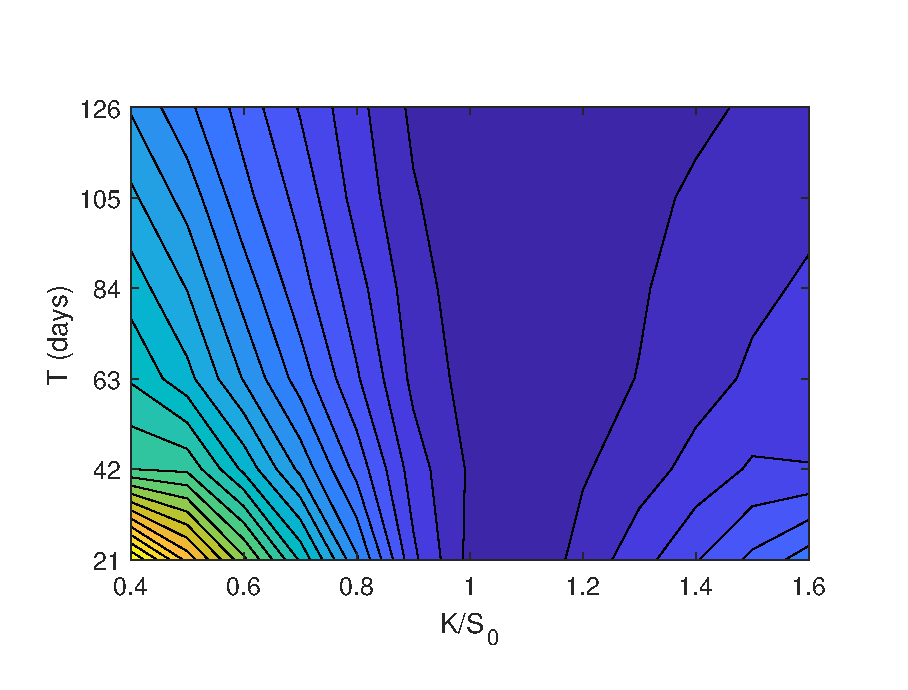
\includegraphics[width=0.49\linewidth,trim={0.2cm 0.5cm 1.25cm 1.55cm},clip]{ImpliedVC.eps}}
  \end{subfigmatrix}
    \caption[Implied volatility surface and corresponding contour plot of the function interpolated linearly between the original data points using Delaunay triangulation.]{Implied volatility surface (left) and corresponding contour plot (right) of the function interpolated linearly between the original data points (blue circles) using Delaunay triangulation.}\label{fig:DupImpV}
\end{figure}   


Observing this interpolated surface we see that its curvature decreases with maturity - the volatility smile becomes less prominent for later maturities.


We now should now be able to generate the \emph{local} volatility surface. To do this, we simply evaluate the interpolated implied volatility surface, as well as all the required gradients, at multiple points $K_j$, $T_i$ to produce the local volatility $\sigma(K_j,T_i)$. The points should be uniformly spaced in a grid - with $K_min$ and $K_max$ being the smallest and largest strike $K_j$ in the grid, with intervals $\Delta K$ between the strikes, and with $T_min$ and $T_max$ the smallest and largest maturity $T_i$, with intervals $\Delta T$. These parameters are shown in \autoref{tab:DupR}.
Interpolating again between these points we are able to generate the local volatility surface, shown in \autoref{fig:DupLocVol}. We now simply need to make a variable change $\sigma(K,T)\implies \sigma(S,t)$ to be able to input this value into eq.\eqref{dupmodds}.


\begin{table}[H]
    \centering
        \renewcommand{\arraystretch}{0.8}
\begin{tabular}{@{}cccccc@{}}
\toprule
$T_{min}$(days) & $T_{max}$(days) & $\Delta T$(days) & $K_{min}$($\EUR$) & $K_{max}$($\EUR$) & \multicolumn{1}{c}{$\Delta K$($\EUR$)}\\ \midrule
21 & 126 & 10.5 & 0.4 & 1.6 & \multicolumn{1}{c}{0.05} \\ \bottomrule
\end{tabular}
  \caption[Parameters used in the interpolation section of Dupire's model.]{Parameters used in the interpolation section of Dupire's model.}
  \label{tab:DupR}
\end{table}


\begin{figure}[H]
  \begin{subfigmatrix}{2}
    \subfigure[$\sigma_{loc}$ surface]{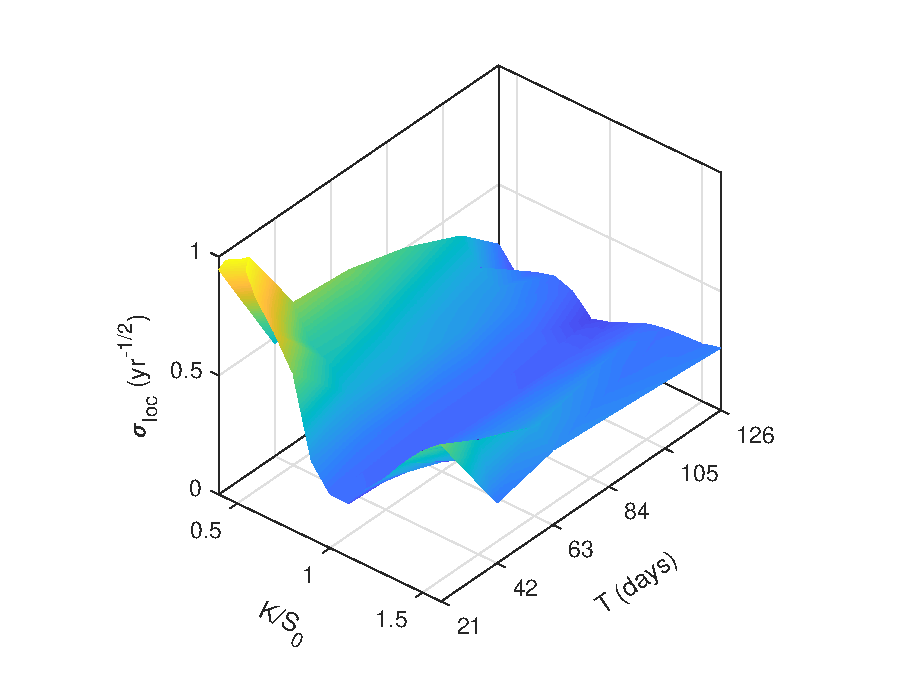
\includegraphics[width=0.49\linewidth,trim={1.7cm 0.45cm 2.cm 0.85cm},clip]{LocalV.eps}}
    \subfigure[$\sigma_{loc}$ contour plot]{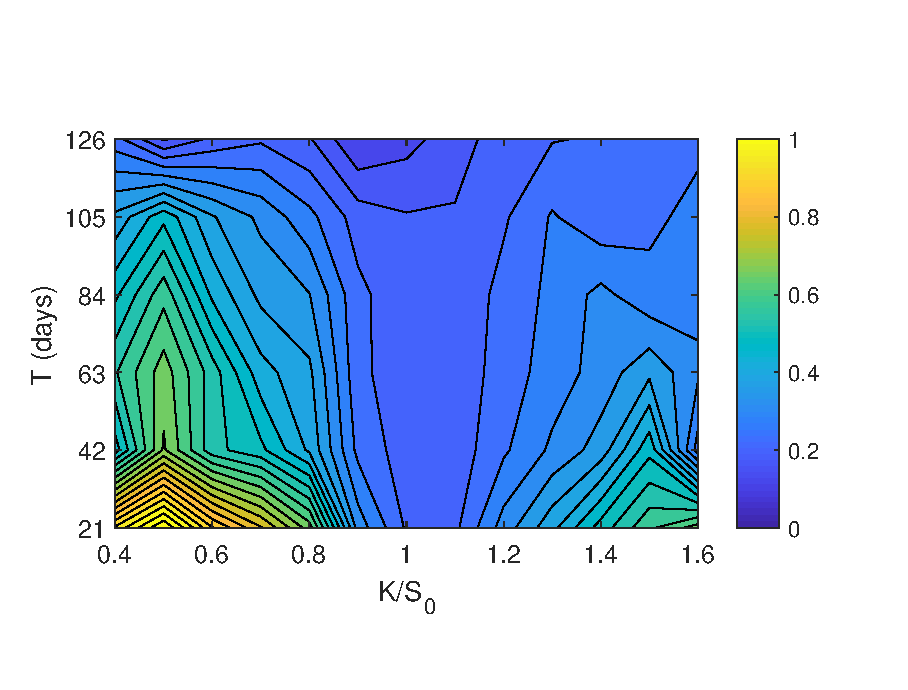
\includegraphics[width=0.49\linewidth,trim={0.2cm 0.5cm 1.25cm 1.55cm},clip]{LocalVC.eps}}
  \end{subfigmatrix}
    \caption[Local volatility surface and corresponding contour plot of the function obtained with Dupire's formula from the interpolated implied volatility surface.]{Local volatility surface (left) and corresponding contour plot (right) of the function obtained with Dupire's formula (eq.\eqref{dupire2}) from the interpolated implied volatility surface in \autoref{fig:DupImpV}.}\label{fig:DupLocVol}
\end{figure}   

Having obtained the local volatility surface, simulating the stock price paths is quite easy. We just need evaluate the surface at the point $(S_i,t_j)$ when we are at the time step $t_j$ of the simulation with a stock price path at $S_i$. To price options, we now simply need to apply the Monte Carlo pricing algorithm. The results of such simulations is shown in \autoref{fig:Dup}, along with the confidence intervals and the original market data. To prevent volatilities from becoming too high we implemented a maximum cutoff value of $\sigma_{max}$=$\SI{1.5}{\year\tothe{-1/2}}$, limiting the volatilities obtained from the surface.

\vspace{\fill}
\newpage

\begin{figure}[H]
  \begin{subfigmatrix}{2}
    \subfigure[$T=21$ days]{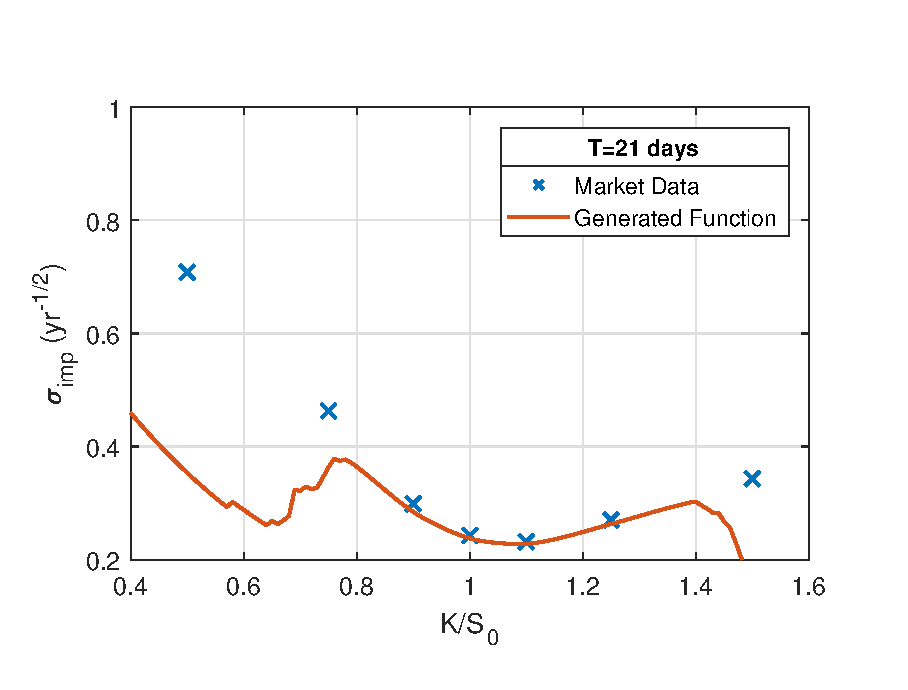
\includegraphics[width=0.49\linewidth,trim={0.25cm 0.45cm 1.1cm 1.4cm},clip]{Dup1.eps}}
    \subfigure[$T=42$ days]{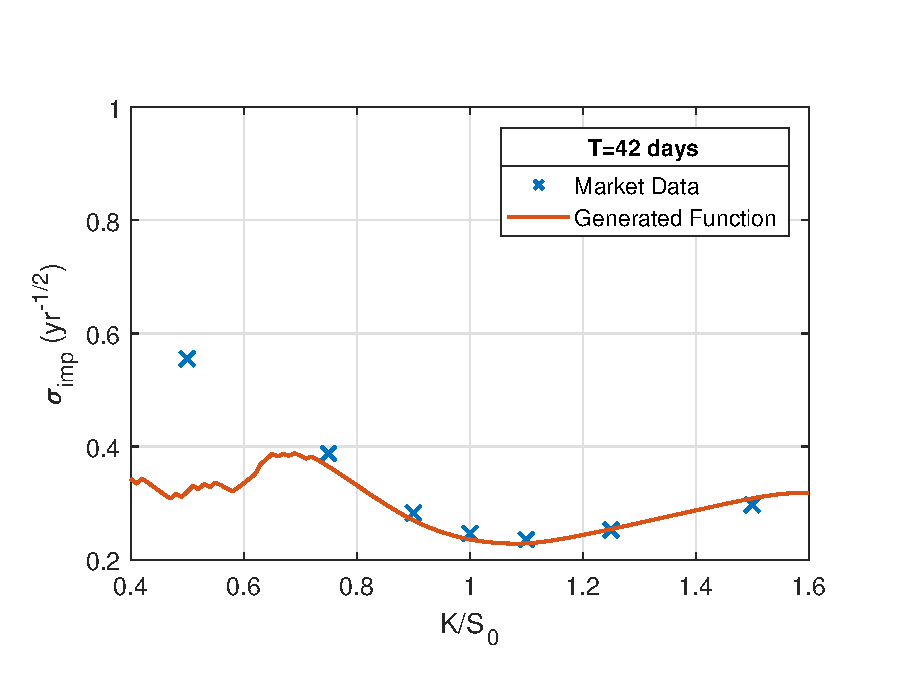
\includegraphics[width=0.49\linewidth,trim={0.25cm 0.45cm 1.1cm 1.4cm},clip]{Dup2.eps}}
    \subfigure[$T=63$ days]{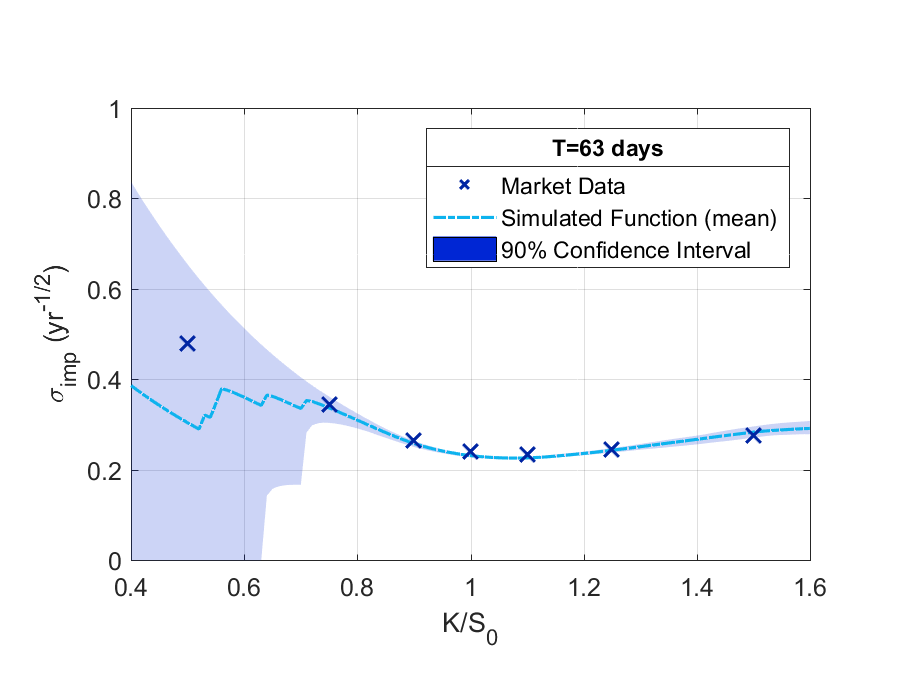
\includegraphics[width=0.49\linewidth,trim={0.25cm 0.45cm 1.1cm 1.4cm},clip]{Dup3.eps}}
    \subfigure[$T=126$ days]{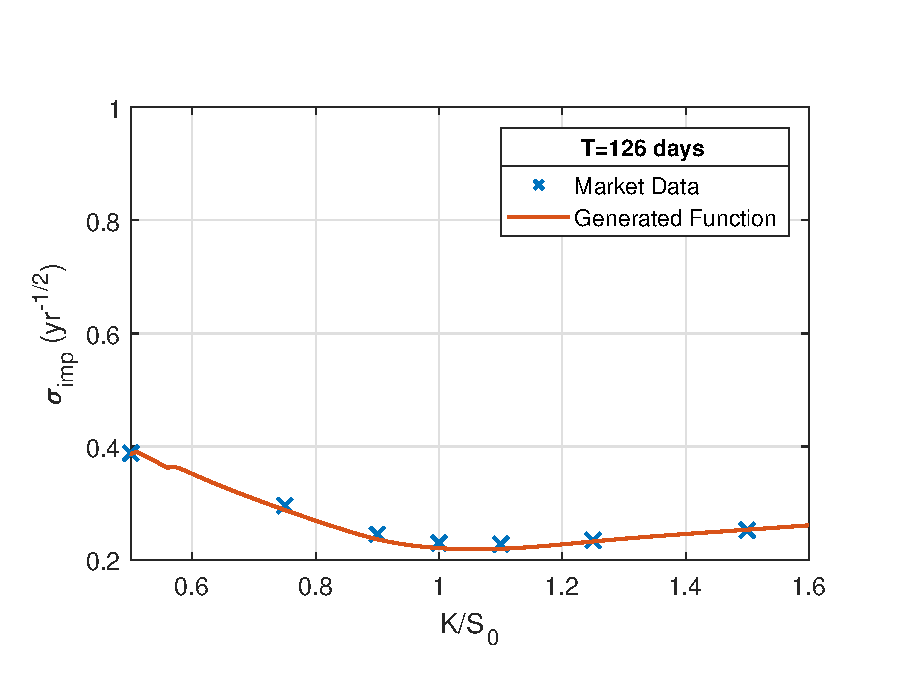
\includegraphics[width=0.49\linewidth,trim={0.25cm 0.45cm 1.1cm 1.4cm},clip]{Dup4.eps}}
  \end{subfigmatrix}
  \caption[Implied volatility functions simulated with Monte Carlo under Dupire's local volatility model with their corresponding 90\% confidence interval, plotted against the original market data.]{Implied volatility functions (light-blue dot-dashed) simulated with Monte Carlo under Dupire's local volatility model with their corresponding 90\% confidence interval, plotted against the original market data (crosses).}
  \label{fig:Dup}
\end{figure}


As before, we now see the very large confidence intervals for very low strikes. The cause of this behavior was identified on the constant volatility model (with independent fits). Also here we can see the low implied volatilities for high strikes in the earliest maturities. This has also already been discussed.

The great improvement of Dupire's model over the constant volatility model is the presence of the implied volatility smiles in the simulated implied volatilities. Furthermore, these smiles follow the market data almost perfectly for strikes near $S_0$.
We can therefore conclude that the model greatly outperforms the constant volatility model presented earlier.

The plots shown in \autoref{fig:Dup} can be thought of as slices of a simulated implied volatility surface. Ideally, this surface would look exactly like the one shown in \autoref{fig:DupImpV}. However, because we are now simulating the prices, there should exist some variation. Furthermore, in the regions where the pricer performs badly (i.e. large strikes for early maturities and low strikes), we expect there to be a very high amount of noise. This simulated surface is shown in \autoref{fig:DupS}, along with the simulated functions of the earlier plots.



\begin{figure}[H]
  \begin{subfigmatrix}{2}
    \subfigure[$\sigma_{imp}$ surface]{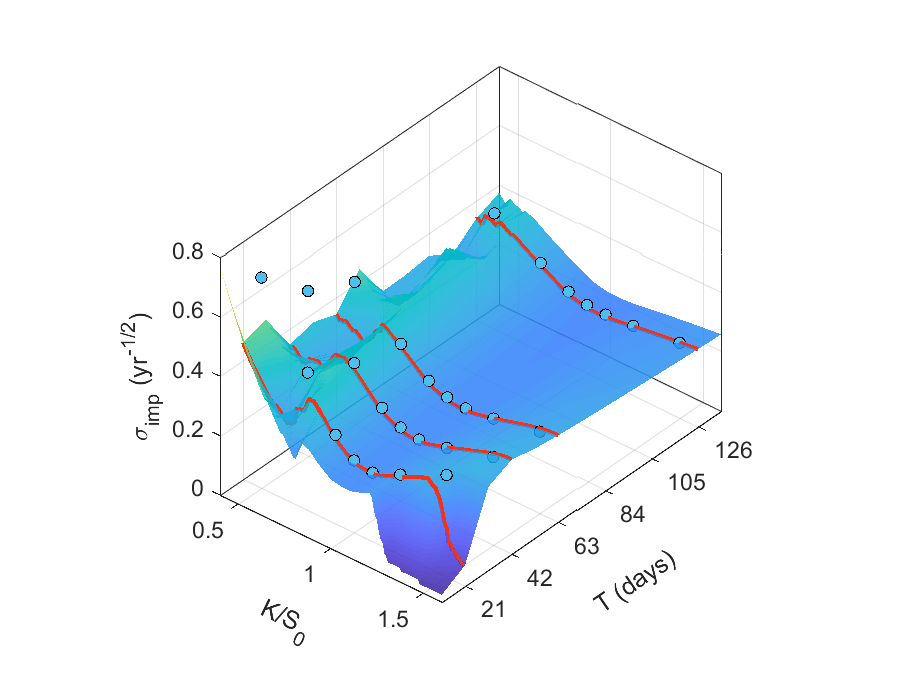
\includegraphics[width=0.49\linewidth,trim={1.7cm 0.45cm 1.9cm 0.85cm},clip]{DupS.eps}}
    \subfigure[$\sigma_{imp}$ contour plot]{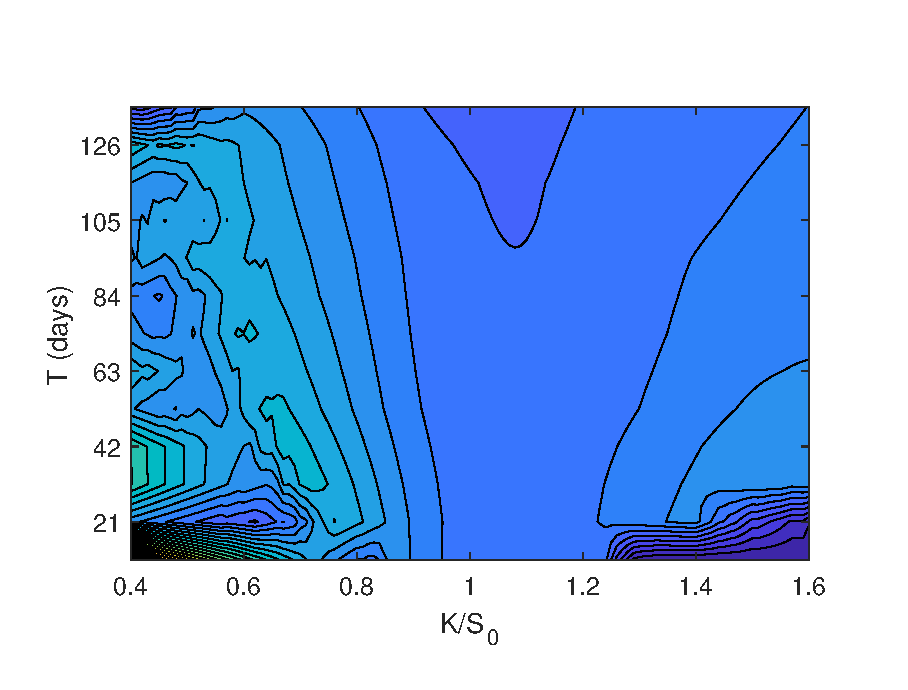
\includegraphics[width=0.49\linewidth,trim={0.2cm 0.5cm 1.25cm 1.55cm},clip]{DupSC.eps}}
  \end{subfigmatrix}
    \caption[Implied volatility surface and corresponding contour plot simulated with Monte Carlo under Dupire's local volatility model plotted against the original market data and the generated functions shown in \autoref{fig:Dup}.]{Implied volatility surface (left) and corresponding contour plot (right) simulated with Monte Carlo under Dupire's local volatility model plotted against the original market data (blue circles) and the generated functions shown in \autoref{fig:Dup} (red dot-dashed lines).}\label{fig:DupS}
\end{figure}   


As expected, the amount of noise is quite overwhelming in the regions where the Monte Carlo pricer performs badly. For the regions where the strike approaches $S_0$, the behavior is quite different and the simulations closely follow the data, as expected.

\vspace{\fill}
\newpage

\begin{table}[H]
\centering
\renewcommand{\arraystretch}{0.8}
\begin{tabular}{@{}ccccSccS@{}}
\toprule
$T$(days) & $K$($\EUR$) & $\sigma_{i,\mathrm{mkt}}$($\SI{}{\year\tothe{-0.5}}$) &  $\sigma_{i,\mathrm{mdl}}$($\SI{}{\year\tothe{-0.5}}$) & \multicolumn{1}{c}{$\mathrm{Error}_{\sigma}(\%)$} & $C_{\mathrm{mkt}}$($\EUR$)&$C_{\mathrm{mdl}}$($\EUR$)& \multicolumn{1}{c}{$\mathrm{Error}_{C}(\%)$}\\ \midrule
\multirow{7}{*}{21} & 0.50 & 0.7082 & 0.2319 & 67.3 & 0.50001 & 0.50000 & 0.003 \\
 & 0.75 & 0.4632 & 0.3740 & 19.3 & 0.25065 & 0.25011 & 0.2 \\
 & 0.90 & 0.2989 & 0.2845 & 4.8 & 0.10439 & 0.10368 & 0.7 \\
 & 1.00 & 0.2425 & 0.2374 & 2.1 & 0.02792 & 0.02734 & 2.1 \\
 & 1.10 & 0.2314 & 0.2276 & 1.7 & 2.42$\times10^{-3}$ & 2.26$\times10^{-3}$ & 6.8 \\
 & 1.25 & 0.2699 & 0.2633 & 2.5 & 5.34$\times10^{-5}$ & 4.06$\times10^{-5}$ & 24.0 \\
 & 1.50 & 0.3433 & 0.1421 & 58.6 & 5.75$\times10^{-7}$ & 0 & 100.0 \\\midrule
\multirow{7}{*}{42} & 0.50 & 0.5556 & 0.3846 & 30.8 & 0.50005 & 0.50000 & 0.01 \\
 & 0.75 & 0.3876 & 0.3683 & 5.0 & 0.25186 & 0.25139 & 0.2 \\
 & 0.90 & 0.2824 & 0.2700 & 4.4 & 0.11069 & 0.10946 & 1.1 \\
 & 1.00 & 0.2461 & 0.2358 & 4.2 & 0.04006 & 0.03838 & 4.2 \\
 & 1.10 & 0.2354 & 0.2286 & 2.9 & 8.52$\times10^{-3}$ & 7.83$\times10^{-3}$ & 8.2 \\
 & 1.25 & 0.2525 & 0.2539 & 0.6 & 6.21$\times10^{-4}$ & 6.46$\times10^{-4}$ & 4.1 \\
 & 1.50 & 0.2968 & 0.3089 & 4.1 & 1.58$\times10^{-5}$ & 2.70$\times10^{-5}$ & 70.3 \\\midrule
\multirow{7}{*}{63} & 0.50 & 0.4789 & 0.3176 & 33.7 & 0.50009 & 0.50000 & 0.02 \\
 & 0.75 & 0.3452 & 0.3355 & 2.8 & 0.25296 & 0.25256 & 0.2 \\
 & 0.90 & 0.2658 & 0.2578 & 3.0 & 0.11533 & 0.11424 & 0.9 \\
 & 1.00 & 0.2401 & 0.2310 & 3.8 & 0.04787 & 0.04606 & 3.8 \\
 & 1.10 & 0.2330 & 0.2253 & 3.3 & 0.01421 & 0.01307 & 8.0 \\
 & 1.25 & 0.2438 & 0.2440 & 0.1 & 1.80$\times10^{-3}$ & 1.81$\times10^{-3}$ & 0.5 \\
 & 1.50 & 0.2749 & 0.2845 & 3.5 & 7.66$\times10^{-5}$ & 11.15$\times10^{-5}$ & 45.7 \\\midrule
\multirow{7}{*}{126} & 0.50 & 0.3878 & 0.3870 & 0.2 & 0.50035 & 0.50035 & 0.001 \\
 & 0.75 & 0.2954 & 0.2876 & 2.6 & 0.25694 & 0.25623 & 0.3 \\
 & 0.90 & 0.2444 & 0.2358 & 3.5 & 0.12716 & 0.12528 & 1.5 \\
 & 1.00 & 0.2295 & 0.2203 & 4.0 & 0.06467 & 0.06207 & 4.0 \\
 & 1.10 & 0.2269 & 0.2190 & 3.5 & 0.02862 & 0.02667 & 6.8 \\
 & 1.25 & 0.2340 & 0.2319 & 0.9 & 7.57$\times10^{-3}$ & 7.31$\times10^{-3}$ & 3.4 \\
 & 1.50 & 0.2521 & 0.2528 & 0.3 & 8.58$\times10^{-4}$ & 8.77$\times10^{-4}$ & 2.2 \\
 \bottomrule
\end{tabular}
  \caption[Comparison between the data obtained by generating $N_{paths}$ paths under Dupire's local volatility model using the Monte Carlo pricing method and the original data.]{Comparison between the data obtained by generating $N_{paths}$ paths under Dupire's local volatility model using the Monte Carlo pricing method and the original data.}
  \label{tab:Dup}
\end{table}










\newpage
\section{Static SABR Model}
As we saw before, the Static SABR model is defined as
\begin{equation}
dS=rSdt+e^{-r(T-t)(1-\beta)}\sigma S^\beta dW_1,
\end{equation}
\begin{equation}
d\sigma=\nu\sigma dW_2,
\end{equation}
\noindent with $\alpha=\sigma(0)$ and with $W_1$ and $W_2$ having a correlation of $\rho$.

The closed form solution, shown in eq.\eqref{sabr}, enables us to obtain the theoretical implied volatilities of options priced under this model and will be used in the calibration process.

Before calibrating the model to the market data, we should study the influence of each parameter of this model on the shape of the implied volatility curve, in order to better interpret the results. This influence is represented in \autoref{fig:SSparam}, where we vary a single parameter at a time, keeping all the others constant, thus directly observing that parameter's influence.


We should note that the influence of the parameters is more complicated than we show here. On the one hand, their impact depends on the maturity. However, for this effect to become evident, we would have to repeat all the plots in \autoref{fig:SSparam} for several maturities, which would simply become too cumbersome and is out of the scope of this thesis.
On the other hand, the parameters have correlated effects on the curve shape. These influences would be quite difficult to represent. Furthermore, they are discussed in the original article by Hagan~\cite{Hagan}, and will, for these reasons, not be discussed here.
That being said, we can still have a general view of each parameter's impact on the curve.

\vspace{\fill}
\newpage

\begin{figure}[H]
  \begin{subfigmatrix}{2}
    \subfigure[Dependence on $\alpha$]{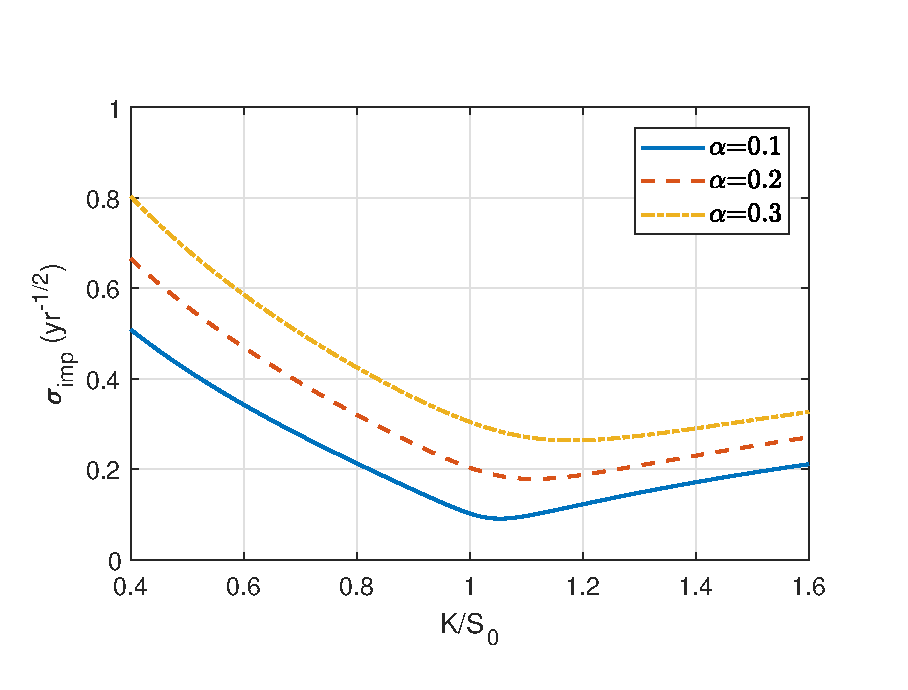
\includegraphics[width=0.49\linewidth,trim={0.25cm 0.45cm 1.1cm 1.4cm},clip]{SSalpha.eps}\label{SSa}}
    \subfigure[Dependence on $\beta$]{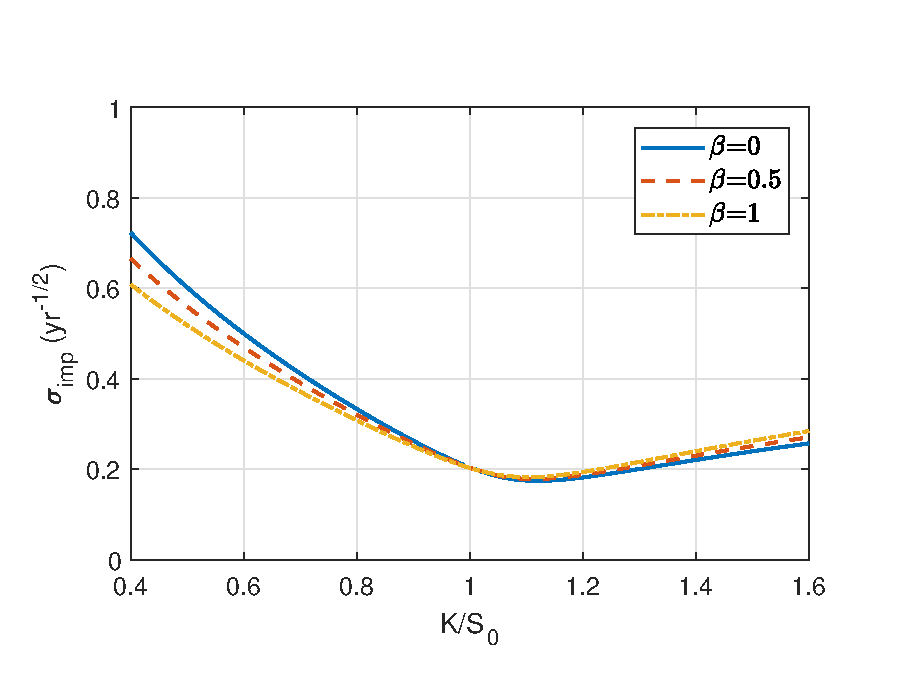
\includegraphics[width=0.49\linewidth,trim={0.25cm 0.45cm 1.1cm 1.4cm},clip]{SSbeta.eps}\label{SSb}}
    \subfigure[Dependence on $\rho$]{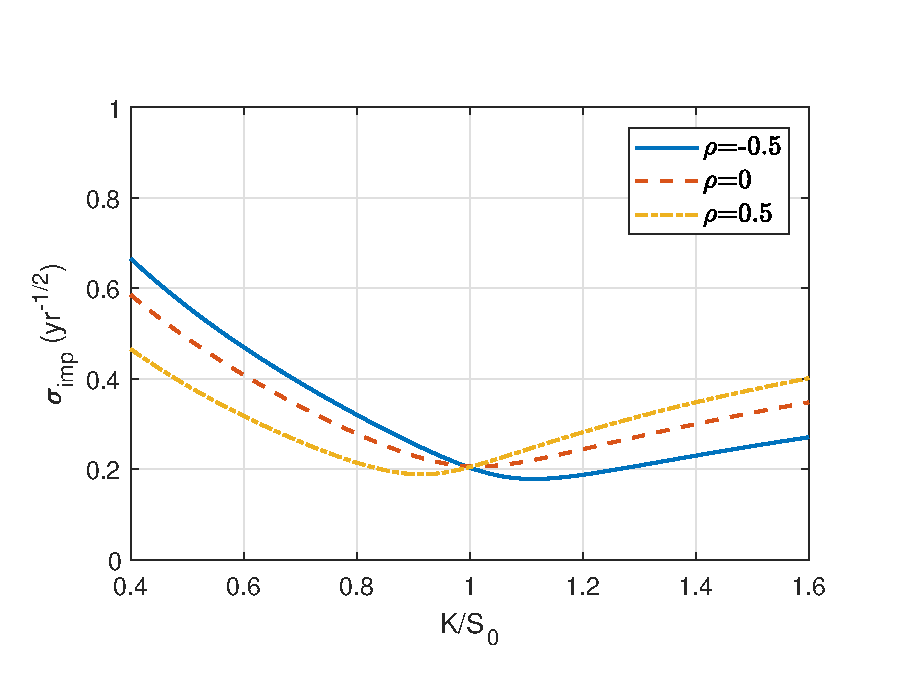
\includegraphics[width=0.49\linewidth,trim={0.25cm 0.45cm 1.1cm 1.4cm},clip]{SSrho.eps}\label{SSr}}
    \subfigure[Dependence on $\nu$]{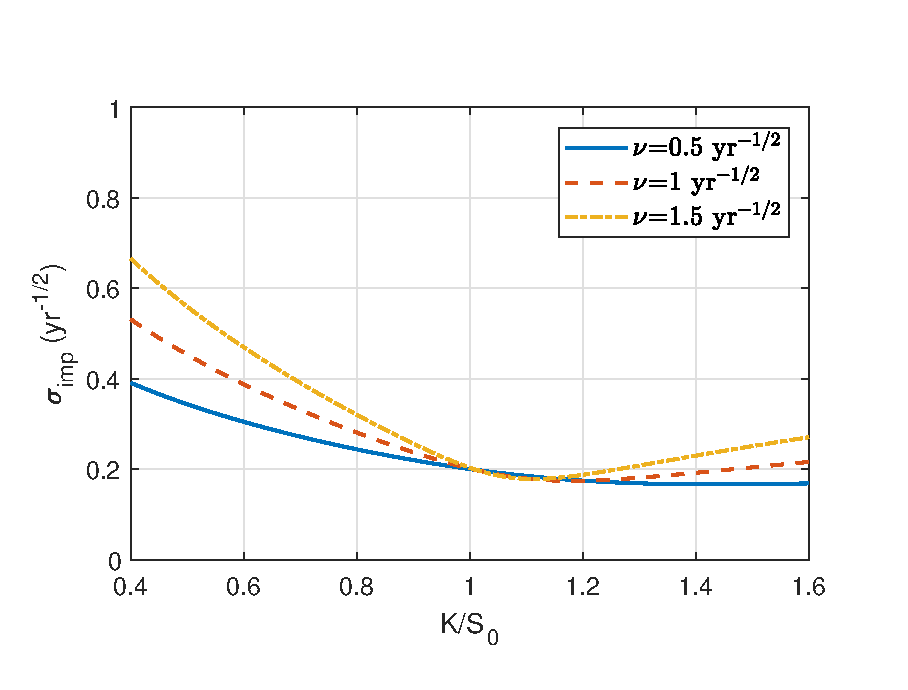
\includegraphics[width=0.49\linewidth,trim={0.25cm 0.45cm 1.1cm 1.4cm},clip]{SSnu.eps}\label{SSn}}
  \end{subfigmatrix}
  \caption[Dependence of the implied volatility curve on each of the Static SABR model parameters.]{Dependence of the implied volatility curve on each of the Static model SABR parameters. The default parameters used were $S_0=1\EUR$, $T=42$ days and $r=0$. Furthermore, on all plots, except when the dependence on a parameter is represented, the parameters used were $\alpha=0.2$, $\beta=1$, $\rho=-0.5$ and $\nu=1.5$.}
  \label{fig:SSparam}
\end{figure}

In Figure \autoref{SSa} we see that the parameter $\alpha$, which corresponds to the initial value of the volatility process, has quite an impact on the implied volatility curve. This parameter essentially controls the height of the curve. This is indeed expected, because the implied volatility and the stochastic (local) volatility are inherently related. Increasing $\alpha$ is expected to shift the volatility process to higher values, thus increasing the implied volatility.

The influence of the parameter $\beta$, which is an exponent in the stock price process, is represented in Figure \autoref{SSb}. The impact of this parameter seems to be almost negligible. Indeed, at a single point in time, the implied volatility curve barely changes, but this parameter becomes very important when time passes and the stock prices move (as they do when being simulated), because it controls how the curve shifts when such movements occur. If the stock price increases, the implied volatility curve at that time should shifts to the right. For $\beta=0$, the curve also shifts downwards, whereas for $\beta=1$ it doesn't. This behavior is studied in detail in the original article by Hagan~\cite{Hagan}.
Despite this, because in Static SABR we are only fitting data for a single maturity, this parameter should barely have any influence in the resulting implied volatility function, though it will become quite relevant in the Dynamic SABR model.

In Figure \autoref{SSr} is represented the effect of the parameter $\rho$, the correlation between the stock price and the volatility processes.
We can see that this parameter impacts the skewness of the implied volatility curve. Because this parameter relates the stock price and volatility, in the case of a negative $\rho$ when the prices increase (decrease), the volatilities decrease (increase), so that options with higher (lower) strikes have lower (higher) associated volatilities. This justifies why we have a lower implied volatility for higher strikes when the correlation is negative.

Finally, the impact of the parameter $\nu$, the volatility of the volatility process, is shown in Figure \autoref{SSn}. This parameter seems to control the curvature of the implied volatility curve. It should be clear that higher values of $\nu$ result in greater changes in the volatility process, enabling, at times, the volatility to become quite large. This allows the stock price process to evolve quite erratically, thus making it easier for stock prices to reach higher values, making high strike options more valuable. This effect pushes their implied volatility upwards. The inverse effect also holds and a low $\nu$ will force the stochastic volatility process to become quite limited, preventing the stock prices from changing too much, and restraining them from reaching high strikes, pulling the implied volatility curve downwards.


We now present the results of the calibration as well as the simulations in \autoref{fig:SS}.

\begin{figure}[H]
  \begin{subfigmatrix}{2}
    \subfigure[$T=21$ days]{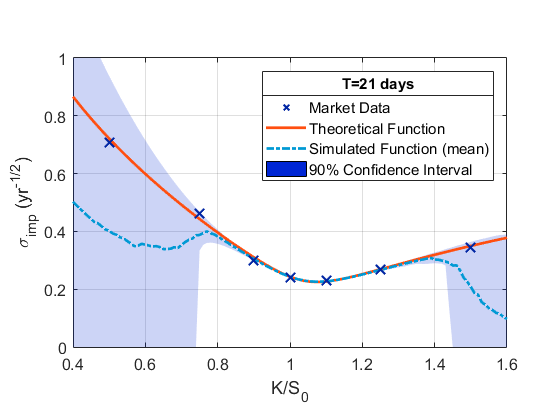
\includegraphics[width=0.49\linewidth,trim={0.25cm 0.45cm 1.1cm 1.4cm},clip]{SSABR1.png}}
    \subfigure[$T=42$ days]{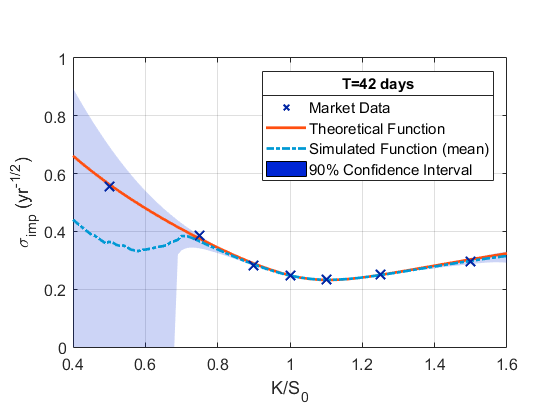
\includegraphics[width=0.49\linewidth,trim={0.25cm 0.45cm 1.1cm 1.4cm},clip]{SSABR2.png}}
    \subfigure[$T=63$ days]{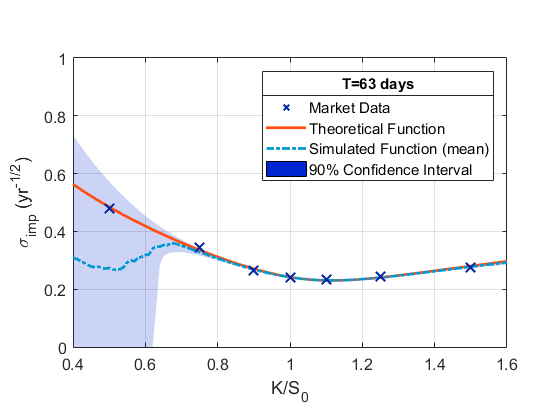
\includegraphics[width=0.49\linewidth,trim={0.25cm 0.45cm 1.1cm 1.4cm},clip]{SSABR3.png}}
    \subfigure[$T=126$ days]{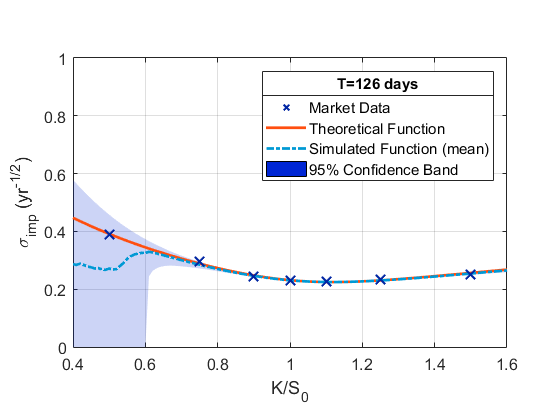
\includegraphics[width=0.49\linewidth,trim={0.25cm 0.45cm 1.1cm 1.4cm},clip]{SSABR4.png}}
  \end{subfigmatrix}
  \caption[Implied volatility functions fitted independently to the implied volatility data for different maturities under the static SABR model, plotted with their respective Monte Carlo simulated functions along with their 90\% confidence intervals.]{Implied volatility functions (red lines) fitted independently to the implied volatility data (crosses) for different maturities under the static SABR model, plotted with their respective Monte Carlo simulated functions (light-blue dot-dashed lines) along with their 90\% confidence intervals (blue region).}
  \label{fig:SS}
\end{figure}

As mentioned before, the Static SABR model is only expected to work for data on options with a single maturity. For this reason, the fits were done independently of one another.
The parameters obtained in the calibration for each of the maturities are shown in \autoref{tab:SSR}.

\begin{table}[H]
    \centering
        \renewcommand{\arraystretch}{0.8}
\begin{tabular}{@{}lccccr@{}}
\toprule
 $T$(days) & $\alpha$ ($\SI{}{\year\tothe{-1/2}}$) & $\beta$ & $\rho$ & $\nu$ & Cost \\ \midrule
21 & 0.2381 & 0.3766 & -0.3760 & 2.1022 & 0.000415 \\
42 & 0.2434 & 0.7362 & -0.3664 & 1.4451 & 0.000166\\
63 & 0.2375 & 0.7750 & -0.3119 & 1.1420 & 0.000102\\
126& 0.2267 & 0.8771 & -0.2383 & 0.8215 & 0.000055\\
\bottomrule
\end{tabular}
  \caption[Fitted parameters for each maturity (fitted independently) under static SABR model.]{Fitted parameters for each maturity (fitted independently) under static SABR model.}
  \label{tab:SSR}
\end{table}


We now analyze the results of this model. Observing the plots in \autoref{fig:SS} we see that the theoretical function, obtained by the closed form solution of the Static SABR model, fits the data extremely well through the whole range of strikes and for each of the maturities.

Though the model seems to fit almost perfectly to the data, the fits may not be very robust. The reason for this is that we have an extremely small amount of data points (7 for each maturity) for the comparatively large number of parameters used (4 parameters in total). This will cause our model to overfit the data.

As for the simulated function, we note that it very closely follows the theoretical curve in the regions around $S_0$, indicating that the Monte Carlo pricer implementation was done correctly. This feature doesn't hold at the high strike region in the first maturity and the low strike regions of all maturities for the same reasons described earlier.

Examining now the calibrated parameters in \autoref{tab:SSR} we first note that the parameter $\alpha$ doesn't seem to vary too much between maturities, which is expected, since it controls the height of the implied volatility curve, which doesn't seem to change too much in the plots.

The parameter $\beta$ appears to change wildly between maturities, though this is not surprising since, as we saw, this parameter doesn't significantly affect the shape of the implied volatility function.

As for the parameter $\rho$, we first note that it is always negative, which is expected from reality. It also seems to decrease with time \hl{why?}.

Finally, the parameter $\nu$ also seems to decrease with time. This is no surprise as the curvature of the implied volatility function is expected to decrease with time, with the function becoming increasingly horizontal.


If we now compare the cost function values of the Static SABR model in \autoref{tab:SSR} with the independently fitted results of the constant volatility assumption in \autoref{tab:ConstVolPar2} we clearly see that they improve very significantly. The cost decreases between 99.2 and 99.4\%, which is an extreme improvement. This is no surprise, since the constant volatility model was expected to perform very badly. These costs should be examined carefully, however, due to the overfitting mentioned earlier - for such a low amount of data relative to the great number of parameters we can find combinations of parameters that decrease the costs significantly, though they might not have any real interpretation.

\begin{table}[H]
\centering
\renewcommand{\arraystretch}{0.8}
\begin{tabular}{@{}ccccSccS@{}}
\toprule
$T$(days) & $K$($\EUR$) & $\sigma_{i,\mathrm{mkt}}$($\SI{}{\year\tothe{-0.5}}$) &  $\sigma_{i,\mathrm{mdl}}$($\SI{}{\year\tothe{-0.5}}$) & \multicolumn{1}{c}{$\mathrm{Error}_{\sigma}(\%)$} & $C_{\mathrm{mkt}}$($\EUR$)&$C_{\mathrm{mdl}}$($\EUR$)& \multicolumn{1}{c}{$\mathrm{Error}_{C}(\%)$}\\ \midrule
\multirow{7}{*}{21} & 0.50 & 0.7082 & 0.7209 & 1.8 & 0.50001 & 0.50002 & 0.001 \\
&0.75 & 0.4632 & 0.4428 & 4.4 & 0.25065 & 0.25047 & 0.1 \\
&0.90 & 0.2989 & 0.3105 & 3.9 & 0.10439 & 0.10501 & 0.6 \\
&1.00 & 0.2425 & 0.2435 & 0.4 & 0.02792 & 0.02804 & 0.4 \\
&1.10 & 0.2314 & 0.2269 & 2.0 & 2.42$\times10^{-3}$ & 2.23$\times10^{-3}$ & 8.0 \\
&1.25 & 0.2699 & 0.2692 & 0.3 & 5.34$\times10^{-5}$ & 5.18$\times10^{-5}$ & 3.0 \\
&1.50 & 0.3433 & 0.3500 & 1.9 & 5.75$\times10^{-7}$ & 8.32$\times10^{-7}$ & 44.7 \\\midrule
\multirow{7}{*}{42} &0.50 & 0.5556 & 0.5631 & 1.4 & 0.50005 & 0.50006 & 0.002 \\
&0.75 & 0.3876 & 0.3751 & 3.2 & 0.25186 & 0.25155 & 0.1 \\
&0.90 & 0.2824 & 0.2891 & 2.4 & 0.11069 & 0.11139 & 0.6 \\
&1.00 & 0.2461 & 0.2481 & 0.8 & 0.04006 & 0.04039 & 0.8 \\
&1.10 & 0.2354 & 0.2322 & 1.4 & 8.52$\times10^{-3}$ & 8.19$\times10^{-3}$ & 3.9 \\
&1.25 & 0.2525 & 0.2497 & 1.1 & 6.21$\times10^{-4}$ & 5.75$\times10^{-4}$ & 7.4 \\
&1.50 & 0.2968 & 0.3033 & 2.2 & 1.58$\times10^{-5}$ & 2.12$\times10^{-5}$ & 33.9 \\\midrule
\multirow{7}{*}{63} &0.50 & 0.4789 & 0.4845 & 1.2 & 0.50009 & 0.50011 & 0.002 \\
&0.75 & 0.3452 & 0.3357 & 2.8 & 0.25296 & 0.25256 & 0.2 \\
&0.90 & 0.2658 & 0.2710 & 2.0 & 0.11533 & 0.11605 & 0.6 \\
&1.00 & 0.2401 & 0.2421 & 0.8 & 0.04787 & 0.04826 & 0.8 \\
&1.10 & 0.2330 & 0.2305 & 1.1 & 0.01421 & 0.01384 & 2.6 \\
&1.25 & 0.2438 & 0.2409 & 1.2 & 1.80$\times10^{-3}$ & 1.68$\times10^{-3}$ & 6.7 \\
&1.50 & 0.2749 & 0.2804 & 2.0 & 7.66$\times10^{-5}$ & 9.56$\times10^{-5}$ & 24.8 \\\midrule
\multirow{7}{*}{126} &0.50 & 0.3878 & 0.3914 & 0.9 & 0.50035 & 0.50038 & 0.006 \\
&0.75 & 0.2954 & 0.2887 & 2.2 & 0.25694 & 0.25633 & 0.2 \\
&0.90 & 0.2444 & 0.2479 & 1.5 & 0.12716 & 0.12794 & 0.6 \\
&1.00 & 0.2295 & 0.2314 & 0.8 & 0.06467 & 0.06522 & 0.8 \\
&1.10 & 0.2269 & 0.2251 & 0.8 & 0.02862 & 0.02817 & 1.6 \\
&1.25 & 0.2340 & 0.2309 & 1.3 & 7.57$\times10^{-3}$ & 7.18$\times10^{-3}$ & 5.2 \\
&1.50 & 0.2521 & 0.2567 & 1.8 & 8.58$\times10^{-4}$ & 9.82$\times10^{-4}$ & 14.5 \\
 \bottomrule
\end{tabular}
  \caption[Comparison between fitted results and original data under static SABR model.]{Comparison between fitted results and original data under static SABR model.}
  \label{tab:SS}
\end{table}







\newpage
\section{Heston Model}
The Heston model is defined as
\begin{equation}
dS=rSdt+\sqrt{\nu}SdW_1,
\end{equation}
\begin{equation}
d\nu=\kappa(\overline{\nu}-\nu)dt+\eta\sqrt{\nu}dW_2,
\end{equation}
\noindent where $\nu_0=\nu(0)$ and with $W_1$ and $W_2$ having a correlation of $\rho$.

The closed form solution, shown in eq.\eqref{CH}, we are able to find the theoretical prices of options priced under this model, which we can easily convert to implied volatilities. These last will be used in the calibration process.

The influence of each parameter of the Heston model on the shape of the implied volatility curve is shown in \autoref{fig:Hparam}.

\vspace{\fill}
\newpage

\begin{figure}[H]
  \begin{subfigmatrix}{2}
    \subfigure[Dependence on $\kappa$]{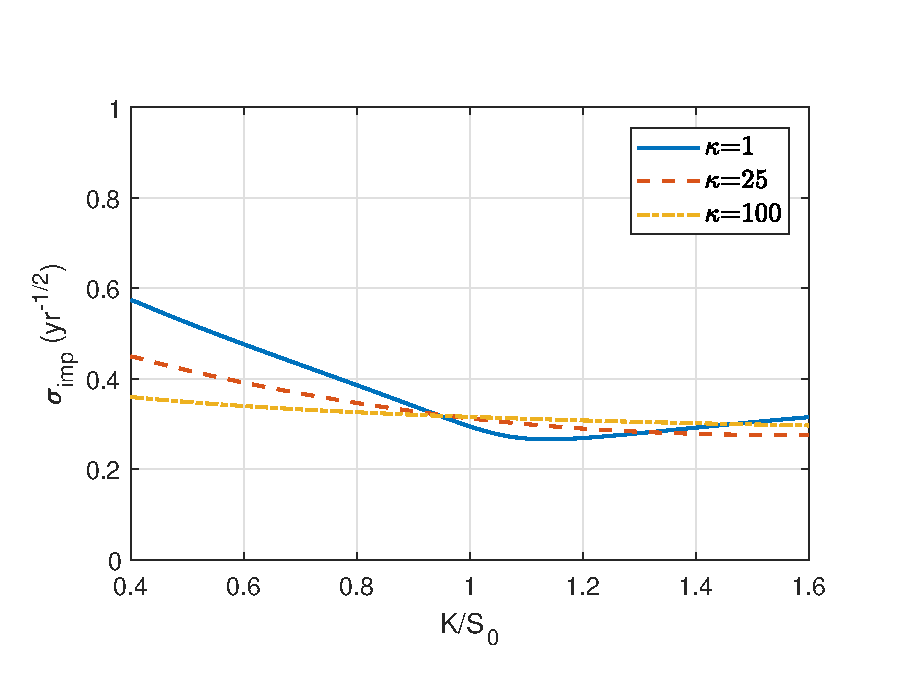
\includegraphics[width=0.49\linewidth,trim={0.25cm 0.45cm 1.1cm 1.4cm},clip]{Hkappa.eps}}
    \subfigure[Dependence on $\overline{\nu}$]{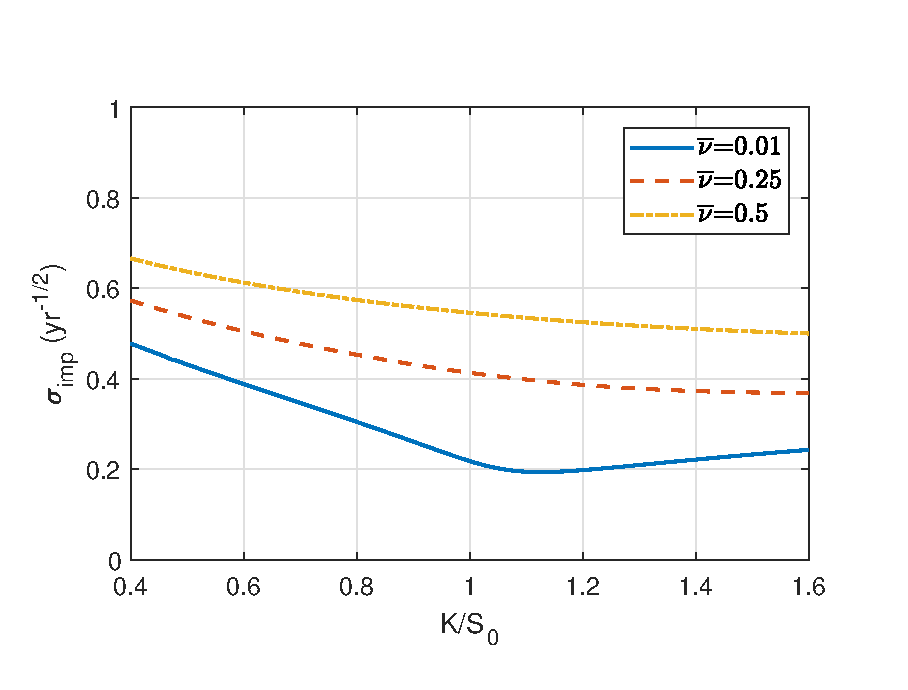
\includegraphics[width=0.49\linewidth,trim={0.25cm 0.45cm 1.1cm 1.4cm},clip]{Hnubar.eps}}
    \subfigure[Dependence on $\nu_0$]{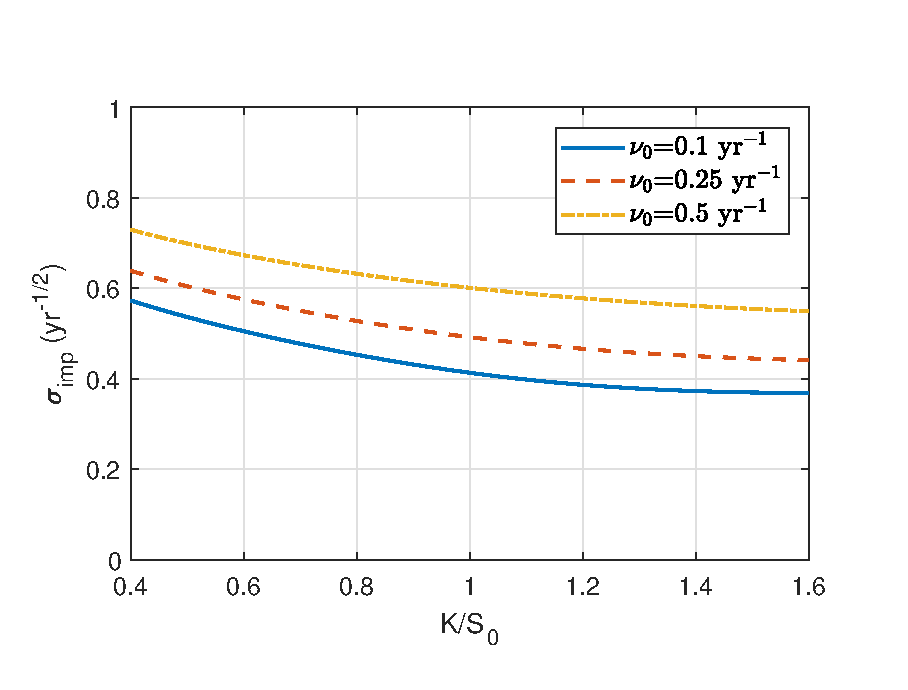
\includegraphics[width=0.49\linewidth,trim={0.25cm 0.45cm 1.1cm 1.4cm},clip]{Hnu0.eps}}
    \subfigure[Dependence on $\eta$]{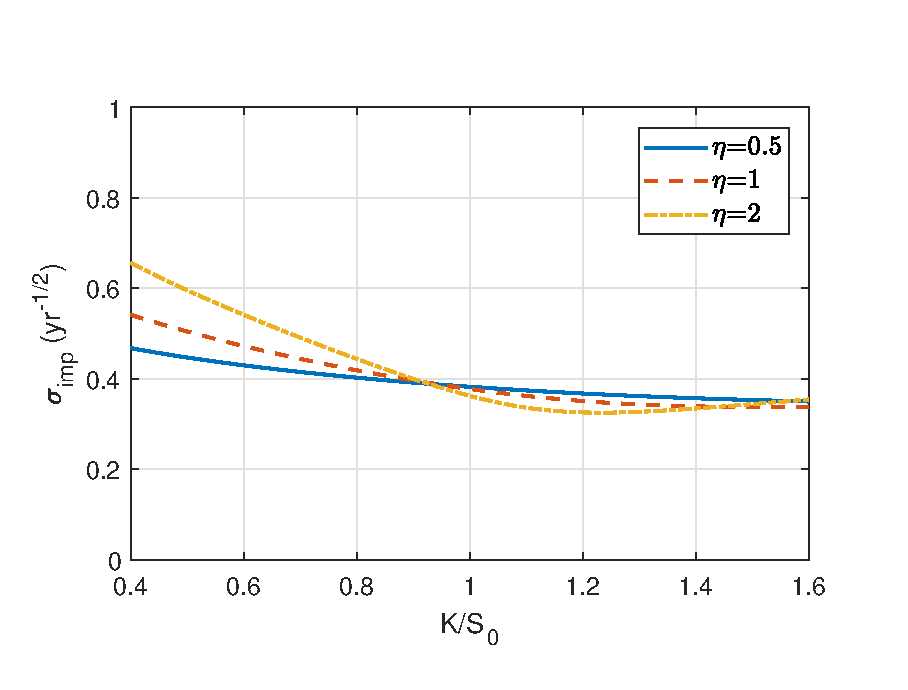
\includegraphics[width=0.49\linewidth,trim={0.25cm 0.45cm 1.1cm 1.4cm},clip]{Heta.eps}}
        \subfigure[Dependence on $\rho$]{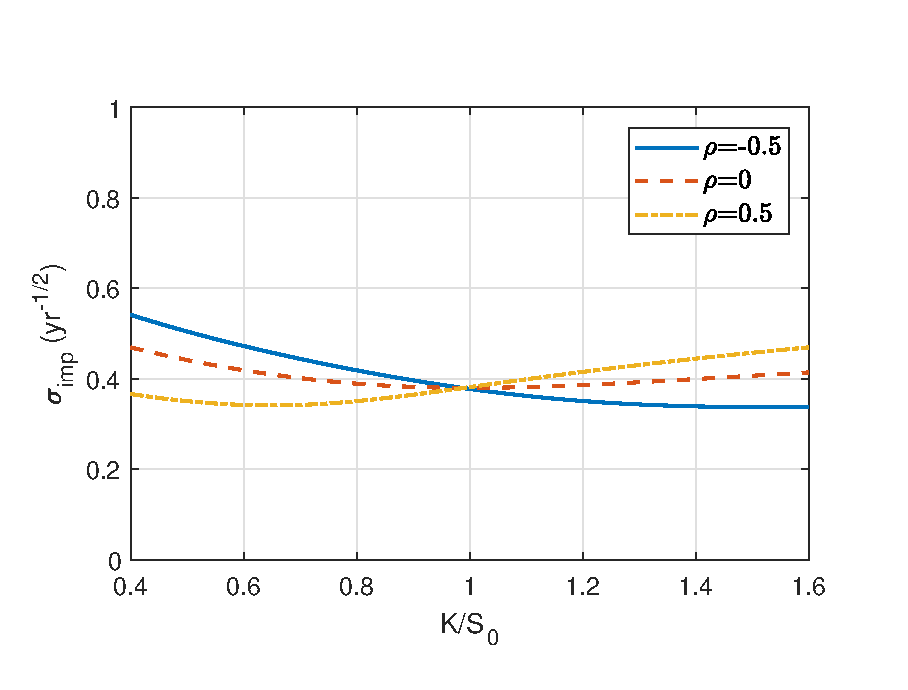
\includegraphics[width=0.49\linewidth,trim={0.25cm 0.45cm 1.1cm 1.4cm},clip]{Hrho.eps}}
  \end{subfigmatrix}
  \caption[Dependence of the implied volatility curve on each of the Heston model parameters.]{Dependence of the implied volatility curve on each of the Heston model parameters. The default parameters used were $S_0=1\EUR$, $T=42$ days and $r=0$. Furthermore, on all plots, except when the dependence on a parameter is represented, the parameters used were $\kappa=10$, $\overline{\nu}=0.1$, $\nu_0=0.1$, $\eta=1$ and $\rho=-0.5$.}
  \label{fig:Hparam}
\end{figure}


\begin{figure}[H]
  \begin{subfigmatrix}{2}
    \subfigure[$T=21$ days]{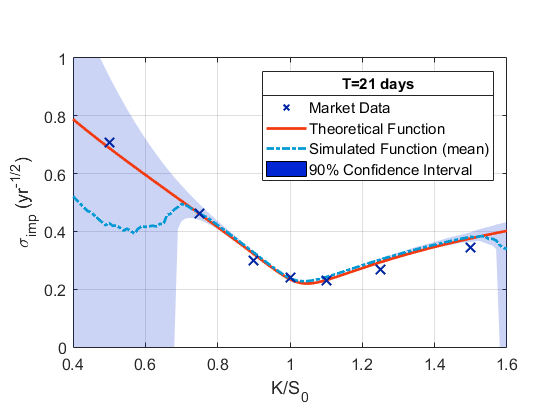
\includegraphics[width=0.49\linewidth,trim={0.25cm 0.45cm 1.1cm 1.4cm},clip]{H1.png}}
    \subfigure[$T=42$ days]{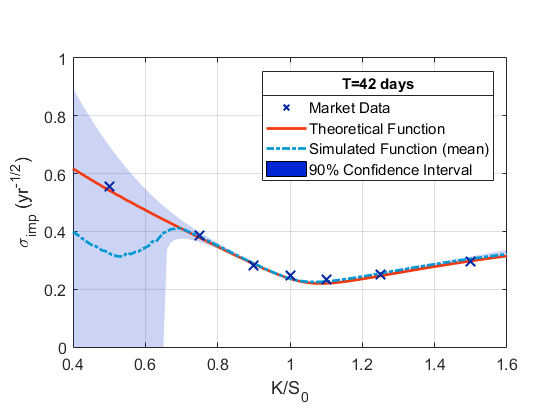
\includegraphics[width=0.49\linewidth,trim={0.25cm 0.45cm 1.1cm 1.4cm},clip]{H2.png}}
    \subfigure[$T=63$ days]{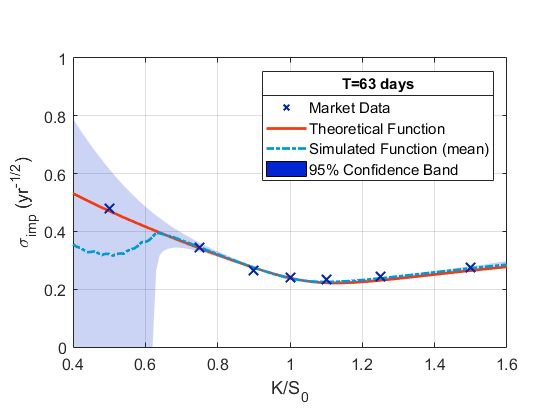
\includegraphics[width=0.49\linewidth,trim={0.25cm 0.45cm 1.1cm 1.4cm},clip]{H3.png}}
    \subfigure[$T=126$ days]{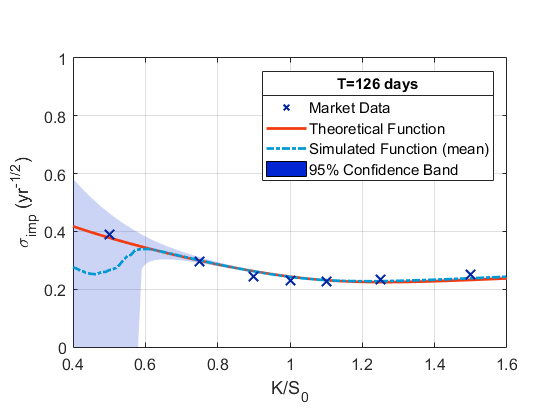
\includegraphics[width=0.49\linewidth,trim={0.25cm 0.45cm 1.1cm 1.4cm},clip]{H4.png}}
  \end{subfigmatrix}
  \caption[Implied volatility functions fitted simultaneously to the implied volatility data for different maturities under the Heston model, plotted with their respective Monte Carlo simulated functions along with their 90\% confidence intervals.]{Implied volatility functions (red lines) fitted simultaneously to the implied volatility data (crosses) for different maturities under the Heston model, plotted with their respective Monte Carlo simulated functions (light-blue dot-dashed lines) along with their 90\% confidence intervals (blue region).}
  \label{fig:H}
\end{figure}




\begin{figure}[H]
  \begin{subfigmatrix}{2}
    \subfigure[$\sigma_{imp}$ surface]{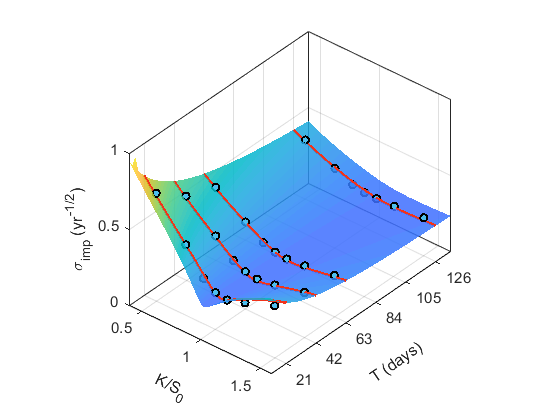
\includegraphics[width=0.49\linewidth,trim={1.7cm 0.45cm 2.35cm 0.85cm},clip]{HS.png}}
    \subfigure[$\sigma_{imp}$ contour plot]{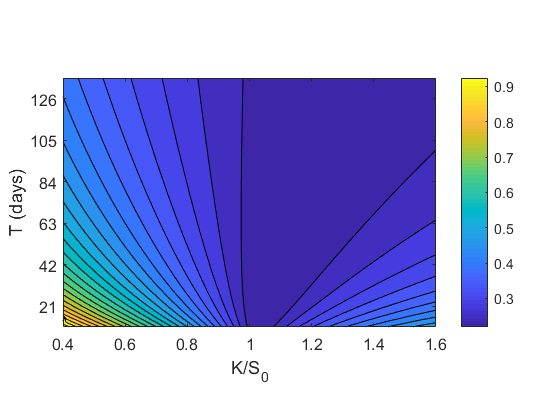
\includegraphics[width=0.49\linewidth,trim={0.2cm 0.5cm 1.25cm 1.55cm},clip]{HSC.png}}
  \end{subfigmatrix}
    \caption[Implied volatility surface and corresponding contour plot of the function fitted simmultaneously to the implied volatility data for different maturities under the Heston model, plotted against the original market data and the fitted functions shown in \autoref{fig:H}.]{Implied volatility surface (left) and corresponding contour plot (right) of the function fitted simmultaneously to the implied volatility data for different maturities under the Heston model, plotted against the original market data (blue circles) and the fitted functions shown in \autoref{fig:H} (red lines).}\label{fig:HS}
\end{figure}   


\begin{figure}[H]
  \begin{subfigmatrix}{2}
    \subfigure[$\sigma_{imp}$ surface]{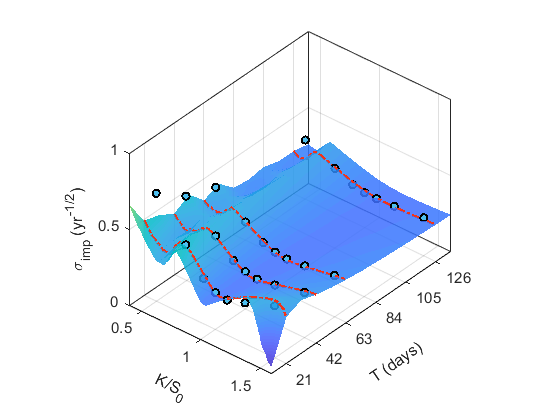
\includegraphics[width=0.49\linewidth,trim={1.7cm 0.45cm 2.35cm 0.85cm},clip]{HSSim.png}}
    \subfigure[$\sigma_{imp}$ contour plot]{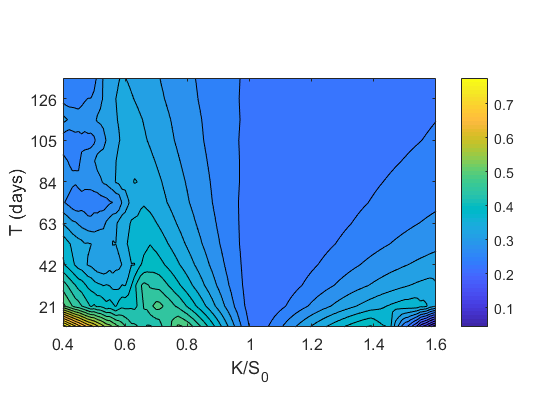
\includegraphics[width=0.49\linewidth,trim={0.2cm 0.5cm 1.25cm 1.55cm},clip]{HSCSim.png}}
  \end{subfigmatrix}
    \caption[Implied volatility surface and corresponding contour plot of the function simulated using the Monte Carlo procedure with the fitted parameters shown in \autoref{tab:HR}, under the Heston model, plotted against the original market data and the simulated functions shown in \autoref{fig:H}.]{Implied volatility surface (left) and corresponding contour plot (right) of the function simulated using the Monte Carlo procedure with the fitted parameters shown in \autoref{tab:HR}, under the dynamic SABR model, plotted against the original market data (blue circles) and the simulated functions shown in \autoref{fig:H} (red dot-dashed lines).}\label{fig:HSSim}
\end{figure} 



\begin{table}[H]
    \centering
        \renewcommand{\arraystretch}{0.8}
\begin{tabular}{@{}lccccr@{}}
\toprule
$\kappa$ & $\overline{\nu}$ & $\nu_0$ & $\rho$ & $\eta$ & Cost \\ \midrule
53.4355 & 0.0653 & 0.1046 & -0.4086 & 6.2554 & 0.002529 \\
\bottomrule
\end{tabular}
  \caption[Fitted parameters for all maturities (fitted simultaneously) under the Heston model.]{Fitted parameters for all maturities (fitted simultaneously) under the Heston model.}
  \label{tab:HR}
\end{table}


\begin{table}[H]
\centering
\renewcommand{\arraystretch}{0.8}
\begin{tabular}{@{}ccccSccS@{}}
\toprule
$T$(days) & $K$($\EUR$) & $\sigma_{i,\mathrm{mkt}}$($\SI{}{\year\tothe{-0.5}}$) &  $\sigma_{i,\mathrm{mdl}}$($\SI{}{\year\tothe{-0.5}}$) & \multicolumn{1}{c}{$\mathrm{Error}_{\sigma}(\%)$} & $C_{\mathrm{mkt}}$($\EUR$)&$C_{\mathrm{mdl}}$($\EUR$)& \multicolumn{1}{c}{$\mathrm{Error}_{C}(\%)$}\\ \midrule
\multirow{7}{*}{21} & 0.50 & 0.7082 & 0.6886 & 2.8 & 0.50001 & 0.50001 & 0.001 \\
 & 0.75 & 0.4632 & 0.4604 & 0.6 & 0.25065 & 0.25062 & 0.01 \\
 & 0.90 & 0.2989 & 0.3216 & 7.6 & 0.10439 & 0.10563 & 1.2 \\
 & 1.00 & 0.2425 & 0.2346 & 3.2 & 0.02792 & 0.02702 & 3.2 \\
 & 1.10 & 0.2314 & 0.2316 & 0.1 & 2.42$\times10^{-3}$ & 2.43$\times10^{-3}$ & 0.3 \\
 & 1.25 & 0.2699 & 0.2935 & 8.7 & 5.34$\times10^{-5}$ & 12.43$\times10^{-5}$ & 132.5 \\
 & 1.50 & 0.3433 & 0.3759 & 9.5 & 5.75$\times10^{-7}$ & 29.58$\times10^{-7}$ & 414.7 \\\midrule
\multirow{7}{*}{42} & 0.50 & 0.5556 & 0.5422 & 2.4 & 0.50005 & 0.50004 & 0.003 \\
 & 0.75 & 0.3876 & 0.3781 & 2.5 & 0.25186 & 0.25162 & 0.1 \\
 & 0.90 & 0.2824 & 0.2873 & 1.7 & 0.11069 & 0.11120 & 0.5 \\
 & 1.00 & 0.2461 & 0.2366 & 3.9 & 0.04006 & 0.03852 & 3.9 \\
 & 1.10 & 0.2354 & 0.2205 & 6.3 & 8.52$\times10^{-3}$ & 7.02$\times10^{-3}$ & 17.6 \\
 & 1.25 & 0.2525 & 0.2463 & 2.4 & 6.21$\times10^{-4}$ & 5.20$\times10^{-4}$ & 16.2 \\
 & 1.50 & 0.2968 & 0.2979 & 0.4 & 1.58$\times10^{-5}$ & 1.66$\times10^{-5}$ & 4.9 \\\midrule
\multirow{7}{*}{63} & 0.50 & 0.4789 & 0.4709 & 1.7 & 0.50009 & 0.50008 & 0.003 \\
 & 0.75 & 0.3452 & 0.3420 & 0.9 & 0.25296 & 0.25282 & 0.1 \\
 & 0.90 & 0.2658 & 0.2748 & 3.4 & 0.11533 & 0.11659 & 1.1 \\
 & 1.00 & 0.2401 & 0.2392 & 0.4 & 0.04787 & 0.04768 & 0.4 \\
 & 1.10 & 0.2330 & 0.2224 & 4.6 & 0.01421 & 0.01265 & 11.0 \\
 & 1.25 & 0.2438 & 0.2310 & 5.2 & 1.80$\times10^{-3}$ & 1.31$\times10^{-3}$ & 27.1 \\
 & 1.50 & 0.2749 & 0.2649 & 3.7 & 7.66$\times10^{-5}$ & 4.97$\times10^{-5}$ & 35.1 \\\midrule
\multirow{7}{*}{126} & 0.50 & 0.3878 & 0.3784 & 2.4 & 0.50035 & 0.50028 & 0.01 \\
 & 0.75 & 0.2954 & 0.2993 & 1.3 & 0.25694 & 0.25732 & 0.1 \\
 & 0.90 & 0.2444 & 0.2626 & 7.5 & 0.12716 & 0.13124 & 3.2 \\
 & 1.00 & 0.2295 & 0.2439 & 6.3 & 0.06467 & 0.06870 & 6.2 \\
 & 1.10 & 0.2269 & 0.2314 & 2.0 & 0.02862 & 0.02973 & 3.9 \\
 & 1.25 & 0.2340 & 0.2248 & 3.9 & 7.57$\times10^{-3}$ & 6.45$\times10^{-3}$ & 14.8 \\
 & 1.50 & 0.2521 & 0.2324 & 7.8 & 8.58$\times10^{-4}$ & 4.45$\times10^{-4}$ & 48.2 \\ 
 \bottomrule
\end{tabular}
  \caption[Comparison between fitted results and original data under the Heston model.]{Comparison between fitted results and original data under the Heston model.}
  \label{tab:H}
\end{table}











\newpage

\section{Dynamic SABR Model}
\begin{figure}[H]
  \begin{subfigmatrix}{2}
    \subfigure[$T=21$ days]{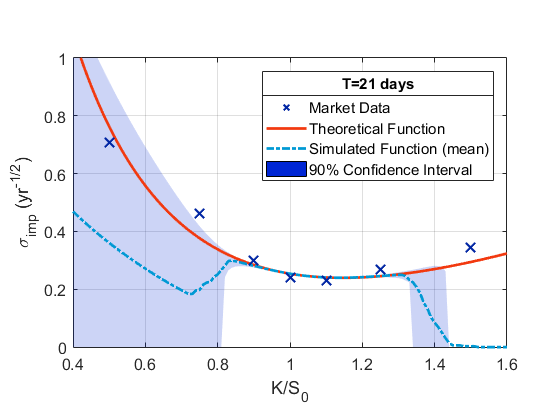
\includegraphics[width=0.49\linewidth,trim={0.25cm 0.45cm 1.1cm 1.4cm},clip]{DS1.png}}
    \subfigure[$T=42$ days]{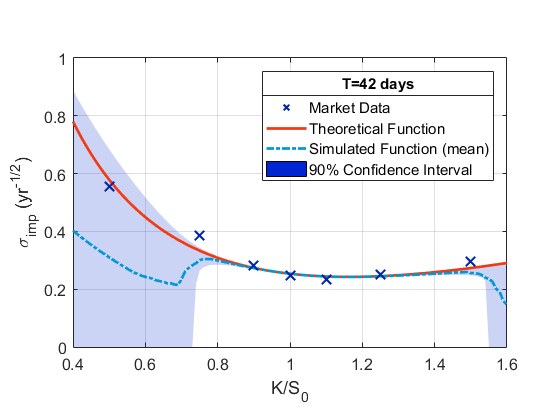
\includegraphics[width=0.49\linewidth,trim={0.25cm 0.45cm 1.1cm 1.4cm},clip]{DS2.png}}
    \subfigure[$T=63$ days]{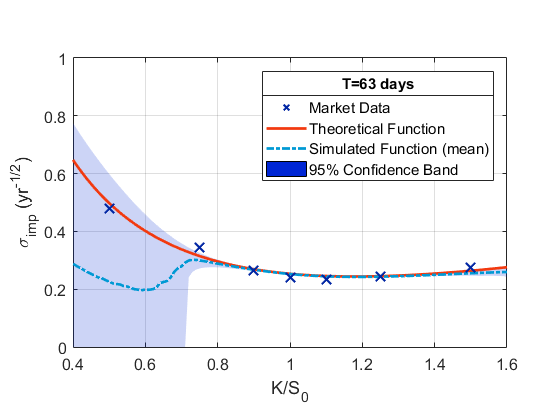
\includegraphics[width=0.49\linewidth,trim={0.25cm 0.45cm 1.1cm 1.4cm},clip]{DS3.png}}
    \subfigure[$T=126$ days]{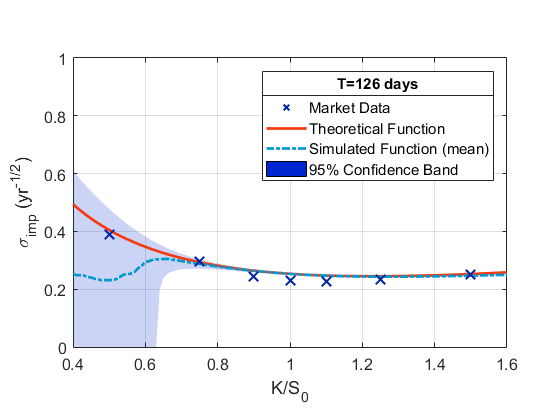
\includegraphics[width=0.49\linewidth,trim={0.25cm 0.45cm 1.1cm 1.4cm},clip]{DS4.png}}
  \end{subfigmatrix}
  \caption[Implied volatility functions fitted simultaneously to the implied volatility data for different maturities under the dynamic SABR model, plotted with their respective Monte Carlo simulated functions along with their 90\% confidence intervals.]{Implied volatility functions (red lines) fitted simultaneously to the implied volatility data (crosses) for different maturities under the dynamic SABR model, plotted with their respective Monte Carlo simulated functions (light-blue dot-dashed lines) along with their 90\% confidence intervals (blue region).}
  \label{fig:DS}
\end{figure}

\vspace{\fill}
\newpage

\begin{figure}[H]
  \begin{subfigmatrix}{2}
    \subfigure[$\sigma_{imp}$ surface]{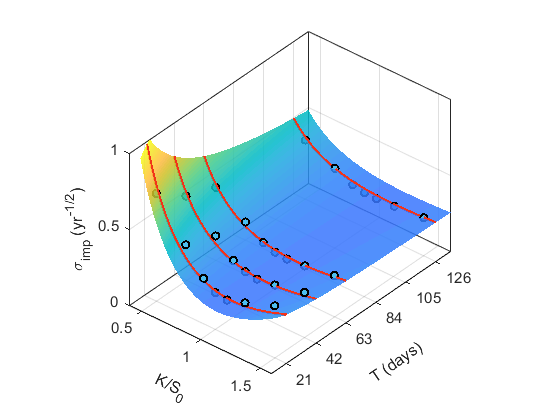
\includegraphics[width=0.49\linewidth,trim={1.7cm 0.45cm 2.35cm 0.85cm},clip]{DSS.png}}
    \subfigure[$\sigma_{imp}$ contour plot]{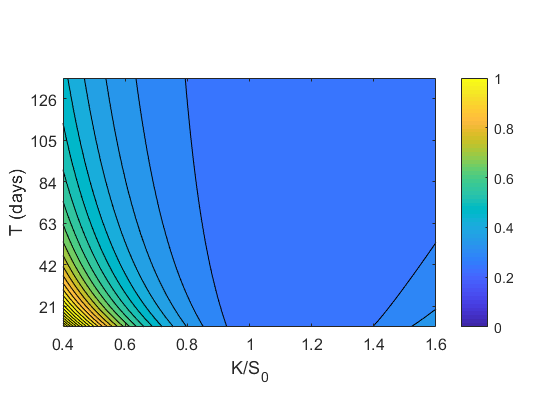
\includegraphics[width=0.49\linewidth,trim={0.2cm 0.5cm 1.25cm 1.55cm},clip]{DSSC.png}}
  \end{subfigmatrix}
    \caption[Implied volatility surface and corresponding contour plot of the function fitted simmultaneously to the implied volatility data for different maturities under the dynamic SABR model, plotted against the original market data and the fitted functions shown in \autoref{fig:DS}.]{Implied volatility surface (left) and corresponding contour plot (right) of the function fitted simmultaneously to the implied volatility data for different maturities under the dynamic SABR model, plotted against the original market data (blue circles) and the fitted functions shown in \autoref{fig:DS} (red lines).}\label{fig:DSS}
\end{figure}   



\begin{figure}[H]
  \begin{subfigmatrix}{2}
    \subfigure[$\sigma_{imp}$ surface]{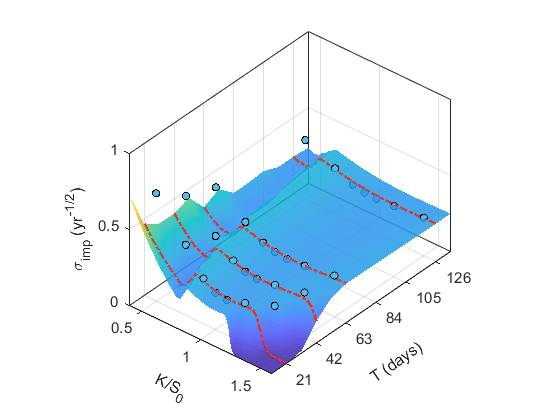
\includegraphics[width=0.49\linewidth,trim={1.7cm 0.45cm 2.35cm 0.85cm},clip]{DSSSim.png}}
    \subfigure[$\sigma_{imp}$ contour plot]{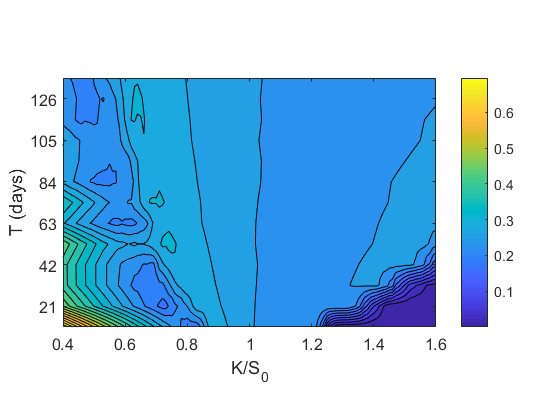
\includegraphics[width=0.49\linewidth,trim={0.2cm 0.5cm 1.25cm 1.55cm},clip]{DSSCSim.png}}
  \end{subfigmatrix}
    \caption[Implied volatility surface and corresponding contour plot of the function simulated using the Monte Carlo procedure with the fitted parameters shown in \autoref{tab:DSR}, under the dynamic SABR model, plotted against the original market data and the simulated functions shown in \autoref{fig:DS}.]{Implied volatility surface (left) and corresponding contour plot (right) of the function simulated using the Monte Carlo procedure with the fitted parameters shown in \autoref{tab:DSR}, under the dynamic SABR model, plotted against the original market data (blue circles) and the simulated functions shown in \autoref{fig:DS} (red dot-dashed lines).}\label{fig:DSSSim}
\end{figure} 


\begin{table}[H]
    \centering
        \renewcommand{\arraystretch}{0.8}
\begin{tabular}{@{}lcccccr@{}}
\toprule
$\alpha$ & $\beta$ & $\rho_0$ & $a$ & $\nu_0$ & $b$ & Cost \\ \midrule
0.2540 & 0.6348 & -0.4166 & 0 & 1.8673 & 41.6943 & 0.0108 \\
\bottomrule
\end{tabular}
  \caption[Fitted parameters for all maturities (fitted simultaneously) under the dynamic SABR model.]{Fitted parameters for all maturities (fitted simultaneously) under the dynamic SABR model.}
  \label{tab:DSR}
\end{table}


\begin{table}[H]
\centering
\renewcommand{\arraystretch}{0.8}
\begin{tabular}{@{}ccccSccS@{}}
\toprule
$T$(days) & $K$($\EUR$) & $\sigma_{i,\mathrm{mkt}}$($\SI{}{\year\tothe{-0.5}}$) &  $\sigma_{i,\mathrm{mdl}}$($\SI{}{\year\tothe{-0.5}}$) & \multicolumn{1}{c}{$\mathrm{Error}_{\sigma}(\%)$} & $C_{\mathrm{mkt}}$($\EUR$)&$C_{\mathrm{mdl}}$($\EUR$)& \multicolumn{1}{c}{$\mathrm{Error}_{C}(\%)$}\\ \midrule
\multirow{7}{*}{21} & 0.50 & 0.7082 & 0.7625 & 7.7 & 0.50001 & 0.50003 & 0.004 \\
 & 0.75 & 0.4632 & 0.3765 & 18.7 & 0.25065 & 0.25012 & 0.2 \\
 & 0.90 & 0.2989 & 0.2843 & 4.9 & 0.10439 & 0.10367 & 0.7 \\
 & 1.00 & 0.2425 & 0.2540 & 4.7 & 0.02792 & 0.02924 & 4.7 \\
 & 1.10 & 0.2314 & 0.2410 & 4.2 & 2.42$\times10^{-3}$ & 2.86$\times10^{-3}$ & 18.0 \\
 & 1.25 & 0.2699 & 0.2454 & 9.1 & 5.34$\times10^{-5}$ & 1.76$\times10^{-5}$ & 67.1 \\
 & 1.50 & 0.3433 & 0.2944 & 14.2 & 57.48$\times10^{-8}$ & 1.86$\times10^{-8}$ & 96.8 \\\midrule
\multirow{7}{*}{42} & 0.50 & 0.5556 & 0.5788 & 4.2 & 0.50005 & 0.50008 & 0.01 \\
 & 0.75 & 0.3876 & 0.3337 & 13.9 & 0.25186 & 0.25074 & 0.4 \\
 & 0.90 & 0.2824 & 0.2740 & 3.0 & 0.11069 & 0.10985 & 0.8 \\
 & 1.00 & 0.2461 & 0.2538 & 3.1 & 0.04006 & 0.04131 & 3.1 \\
 & 1.10 & 0.2354 & 0.2445 & 3.9 & 8.52$\times10^{-3}$ & 9.49$\times10^{-3}$ & 11.3 \\
 & 1.25 & 0.2525 & 0.2455 & 2.8 & 6.21$\times10^{-4}$ & 5.07$\times10^{-4}$ & 18.3 \\
 & 1.50 & 0.2968 & 0.2736 & 7.8 & 15.83$\times10^{-6}$ & 4.72$\times10^{-6}$ & 70.2 \\\midrule
\multirow{7}{*}{63} & 0.50 & 0.4789 & 0.4980 & 4.0 & 0.50009 & 0.50014 & 0.01 \\
 & 0.75 & 0.3452 & 0.3150 & 8.8 & 0.25296 & 0.25182 & 0.5 \\
 & 0.90 & 0.2658 & 0.2695 & 1.4 & 0.11533 & 0.11585 & 0.4 \\
 & 1.00 & 0.2401 & 0.2537 & 5.7 & 0.04787 & 0.05057 & 5.6 \\
 & 1.10 & 0.2330 & 0.2460 & 5.6 & 0.01421 & 0.01619 & 13.9 \\
 & 1.25 & 0.2438 & 0.2455 & 0.7 & 1.80$\times10^{-3}$ & 1.87$\times10^{-3}$ & 3.8 \\
 & 1.50 & 0.2749 & 0.2642 & 3.9 & 7.66$\times10^{-5}$ & 4.81$\times10^{-5}$ & 37.2 \\\midrule
\multirow{7}{*}{126} & 0.50 & 0.3878 & 0.4050 & 4.4 & 0.50035 & 0.50051 & 0.03 \\
 & 0.75 & 0.2954 & 0.2935 & 0.6 & 0.25694 & 0.25677 & 0.1 \\
 & 0.90 & 0.2444 & 0.2645 & 8.2 & 0.12716 & 0.13168 & 3.6 \\
 & 1.00 & 0.2295 & 0.2537 & 10.5 & 0.06467 & 0.07147 & 10.5 \\
 & 1.10 & 0.2269 & 0.2477 & 9.1 & 0.02862 & 0.03382 & 18.2 \\
 & 1.25 & 0.2340 & 0.2452 & 4.8 & 7.57$\times10^{-3}$ & 9.05$\times10^{-3}$ & 19.6 \\
 & 1.50 & 0.2521 & 0.2528 & 0.3 & 8.58$\times10^{-4}$ & 8.77$\times10^{-4}$ & 2.3 \\
 \bottomrule
\end{tabular}
  \caption[Comparison between fitted results and original data under the dynamic SABR model.]{Comparison between fitted results and original data under the dynamic SABR model.}
  \label{tab:DS}
\end{table}





\section{Mishaps Found in Implementation}
\hl{mention the oscillating errors in heston due to integration}

\hl{sabr negative prices: S can become negative, so we must input the restriction S=max(S,0)}

\hlc[green]{in the tables show only one maturity and show the simulation implied vols, deleting the option prices (or showing in a different table)}

\hlc[green]{create a cost function for the simulated volatility functions besides the already existing cost for the theoretical values, in order to compare dupire's model}

\hlc[green]{put the same limits on the contour plots of all the surfaces for comparability}

\hlc[red]{why is the coupled constant implied volatility the average of the independent fits of the constant implied vols?}



\newpage


\hl{check notation:}

$\sigma_{i,\mathrm{mkt}}$ vs $\sigma_{imp,\mathrm{mkt}}$;

\hl{put units in fitted parameters}

\hl{talk about the problem of volatility with sabr (switch volatility and price in code)}

\hl{plot the decaying functions of rho and nu on the dynamic sabr model}



\hl{in the plots of the chapters background and implementation, use dashed and dot-dashed lines}

\hl{save files as .png}

\hl{change labels from "simulated function" to something else}

\hl{explain the effect of barrier level on the price of barrier options}


\hl{!!!mention the implied vol sensitivity to option price but changing maturity.}

\hl{barriers might be broken in between time steps in the simulations. because we are discretizing the time and not using continuous time, this introduces an error}

\hl{check with Claude if BNPP data assumes a 0 interest rate or not}

\hl{explain why stock prices follow a GBM}

\hl{how is extrapolation done in dupires model}

\hl{put numerical formula for gradients}

\hl{explain why we have implied volatility smile: when things go bad/well, they go really bad/well.}

\hl{interest rate is not necessarily constant in black scholes! we just assume it is a known function of time}

\hl{check "casas decimais" in the parameters tables (in particular for the cost function value)}